\chapter{Din\'amica}
\label{cha:dinamica}

\section{Sistemas inerciales}

\subsection{Transformaciones de Galileo}

Los vectores como la velocidad, la aceleración o el moméntum
son independientes de sistemas de referencia en
reposo. 
Considere ahora dos sistemas de referencia con $S:(x,y,z,t)$ en reposo
y $S':(x',y',z',t')$ moviéndose a velocidad constante
$\mathbf{V}$. 
Como hipótesis, asumamos que el patrón de medida no se afecta al
encontrarse en el sistema de referencia en movimiento, y que el tiempo
transcurre de la misma forma en los dos sistemas. 
Estas hipótesis son válidas si $v\ll c$ y serán reevaluadas cuando se
formule la Relatividad Especial en el
Capítulo~\ref{cha:relatividad-especial}. 
Entonces,
\begin{align}
  t=t'\qquad v\ll c\,.
\end{align}
Sea $\mathbf{r}$ el vector de posición de un cuerpo relativo al
primer sistema de referencia, y $\mathbf{r}'$ su vector de posición
relativo al segundo.
Asumiendo que los sistemas de referencia coinciden en el tiempo
$t=t'=0$, entonces
\begin{align}
  \mathbf{r}(t)=\mathbf{r}'(t)+\mathbf{R}(t)\,.
\end{align}
donde el sistema de coordenadas primado se mueve con velocidad
$\mathbf{V}$ a largo de $\mathbf{R}$:
\begin{align}
  \mathbf{R}(t)=\mathbf{V}\, t\,,
\end{align}
y como $d\mathbf{V}/dt=0$. Entonces
\begin{align}
\label{eq:rp}
  \mathbf{r}=&\mathbf{r}'+\mathbf{V}t\nonumber\\
  \mathbf{r}'=&\mathbf{r}-\mathbf{V}t\,.
\end{align}

En el caso especial de un sistema de referencia moviéndose a lo largo
del eje $x$, tenemos
\begin{align}
  \mathbf{r}'=\mathbf{r}-V t\,\hat{\mathbf{i}}\,,
\end{align}
o
\begin{align}
  t'=&t\nonumber\\
  x'=&x-vt\nonumber\\
  y'=&y\nonumber\\
  z'=&z\,.
\end{align}
\begin{align}
  \begin{pmatrix}
    t'\\
    x'\\
    y'\\
    z'\\
  \end{pmatrix}=
  \begin{pmatrix}
    1&0&0&0\\
    -V&1&0&0\\
    0&0&1&0\\
    0&0&0&1\\
  \end{pmatrix}
  \begin{pmatrix}
    t\\
    x\\
    y\\
    z\\
  \end{pmatrix}
\end{align}
A estas relaciones se les conoce como reglas de transformación, y en
este caso corresponden a las \emph{Transformaciones de Galileo}.
Por ejemplo, las traslaciones espaciales son un caso particular de la
ecuación para $x'$ cuando $x'=x+a$ con $a$ una distancia constante.
Si el cuerpo se mueve con velocidad $\mathbf{v}(t)$ relativo al
sistema $S$, podemos hallar su velocidad relativa al sistema $S'$
derivando la ec.~\eqref{eq:rp} con respecto al tiempo y teniendo en
cuenta que la velocidad $\mathbf{V}$ no cambia con el tiempo
\begin{align}
\frac{d\mathbf{r}'}{dt}=&\frac{d\mathbf{r}}{dt}-\frac{d}{dt}\left(\mathbf{V}t\right)\nonumber\\
  \mathbf{v}'(t)=&\mathbf{v}(t)-\mathbf{V}\,.
\end{align}
Pero para la aceleración:
\begin{align}
  \mathbf{a}'=\mathbf{a}\,,
\end{align}
de modo que si la velocidad relativa entre los sistemas es constante,
la aceleración de un objeto vista desde los dos sistemas de referencia
es la misma.

Los sistemas de referencia moviéndose a velocidad constante se
relacionan entre sí a través de las transformaciones de Galileo y
reciben el nombre de sistemas inerciales: un sistema de coordenadas
inercial, es un sistema de coordenadas que se mueve a velocidad
constante.
Como la aceleración es la misma desde todos los sistemas inerciales,
los diferentes sistemas inerciales observan los mismos cambios en la
velocidad de un cuerpo en movimiento y por lo tanto las Leyes de la
física responsables de las fuerzas que están cambiando la velocidad el
objeto deben ser independientes de los sistemas inerciales con
respecto al cual se mida. 
El movimiento tiene sentido solamente con respecto a un sistema
particular de coordenadas, y al momento de describir el movimiento es
esencial especificar el sistema de coordenadas que se este usando. De
este forma podemos formular el:

\textbf{Principio de relatividad:} Las leyes de la física mantienen su forma en distintos sistemas inerciales.

Además podemos reformular la Primera Ley de Newton:

\textbf{Primera Ley de Newton}: Los cuerpos aislados se mueven
uniformemente con respecto a sistemas inerciales.

Un cuerpo sobre el que no actúan fuerzas se llama \emph{cuerpo libre}.

\section{Principios de la Mecánica}
La homogeneidad e isotropía del espacio, y la homogeneidad del tiempo
son ejemplos de transformaciones continuas que forman lo que
matemáticamente se conocen como Grupos de Lie.


Las cantidades físicas pueden sufrir transformaciones de traslaciones
o rotaciones bajo grupos continuos, pero las leyes físicas deben
mantener su forma después de estas transformaciones. 
Más aún, \textbf{El Teorema de Noether} establece que por cada
transformación continua existe alguna carga conservada. 
Aunque no demostraremos este teorema si lo ilustraremos con ejemplos
específicos. 
En mecánica este teorema da lugar a tres leyes de conservación
importantes, resumidas en la Tabla~\ref{tab:tn}

\begin{frame}
  
\begin{table}
  \centering
  \begin{tabular}{|p{5cm}|l|p{5cm}|}\hline{}
    \textbf{Transformación} &\textbf{Ley Física}  &  \textbf{Cantidad conservada}\\\hline
Traslaciones espaciales & Principio de moméntum & Moméntum\\
Traslación temporal & Principio de Energía & Energía\\
Rotaciones & Principio de momentum angular & Moméntum angular\\
Transformaciones de Galileo&Principio de Relatividad & 
Movimiento uniforme del centro de masa\\\hline
  \end{tabular}
  \caption{Implicaciones del teorema de Noether en mecánica}
  \label{tab:tn}
\end{table}
\end{frame}

En este curso estableceremos y usaremos cada uno de estos tres principios.

\section{Principio de Moméntum}

Primero algunas definiciones:

\subsection{Sistema y entorno}

Un \emph{sistema} puede estar conformada por uno o más objetos. Todo lo que no está incluido en el sistema es parte del \textbf{entorno}



\subsection{Segunda Ley de Newton}

\begin{frame}
  %\begin{block}%
{El Principio de Moméntum}, que también se conoce como la Segunda Ley de Newton es:
\begin{align}
\label{eq:ppiomomentum}
  \Delta\mathbf{p}=\mathbf{F}_{\text{neta}}\Delta t
\end{align}
  %\end{block}
\end{frame}
%Falta discusión de la notas del cuaderno aquí

El cambio de moméntum de un sistema es igual a la fuerza neta actuando sobre el sistema veces la duración de la interacción. 

El cambio en el intervalo de tiempo debe ser suficientemente pequeño como para que la fuerza sea aproximadamente constante durante este intervalo de tiempo.

Para entender cada término de está ecuación, consideremos cada cantidad involucrada. 
\begin{itemize}
\item Cambio en el moméntum $\Delta\mathbf{p}$: Puede involucrar
  \begin{itemize}
  \item Cambio en la magnitud del moméntum
  \item Cambio en la dirección del moméntum
  \item Cambio en ambos
  \end{itemize}
\item Fuerza $\mathbf{F}$: La fuerza cuantifica la cantidad de interacción entre dos objetos. Como la fuerza tiene una determinada magnitud y se ejerce en una dirección, entonces es un vector

Ejemplos:
\begin{itemize}
\item Fuerza repulsiva entre un protón y otro protón.
\item La fuerza gravitacional atractiva que la tierra ejerce sobre usted.
\item La fuerza que un resorte comprimido ejerce sobre su mano.
\item La fuerza en una nave espacial de los gases expandiéndose en la
  maquinaria del cohete.
\end{itemize}

%hacer diagramas de resortes
\item Las fuerza neta actuando en un sistema en un instante es el vector de
suma de todas la fuerzas ejercidas sobre el sistema por todos los
objetos del entorno, las cuales son llamadas fuerzas externas. Puede
haber fuerzas internas al sistema, ejercidas por un objeto del sistema
en otro objeto del sistema, pero tales fuerzas internas no pueden
cambiar el moméntum del sistema. Veremos en detalle el por qué en
el siguiente capítulo, pero la idea básica es que las fuerzas internas
se cancelan entre si: una fuerza que el objeto 1 hace sobre el objeto
2 en el sistema, cambia el moméntum del objeto 2. Pero el objeto 2
ejerce una fuerza en dirección opuesta en el objeto 1 que cambia el
moméntum del objeto de la forma opuesta, de modo que el cambio en el
moméntum de los dos objetos suma cero. 

\end{itemize}




  

\begin{frame}
  \begin{block}%
{Pregunta:} Una bola cayendo hacia la tierra consiste de muchos
  átomos. Cada átomo en la bola ejerce fuerzas en sus átomos vecinos
  de la bola, la tierra ejerce fuerzas en cada átomo de la bola, y el
  aire ejerce fuerzas en los átomos de la superficie de la
  bola. Tomando la bola como el sistema, y la tierra y el aire como el
  entorno, ¿cuales de estas fuerzas son externas y cuales internas?.
    
  \end{block}

  
\end{frame}

\begin{frame}
\begin{itemize}
  \item     \alert{La tierra y el aire} son parte del entorno, de modo que las fuerzas
    ejercidas por la tierra el aire son ambas \alert{externas}.
  \item Las fuerzas \alert{inter-atómicas} de los átomos de la bola son
    fuerzas \alert{internas} que no contribuyen a la fuerza neta $\mathbf{F}_{\text{neta}}$
  \end{itemize}
  
\end{frame}

\begin{frame}
  La cantidad de interacción afectando un objeto incluye tanto la \alert{intensidad de la interacción} ($\mathbf{F}_{\text{neta}}$) y la \alert{duración} $\Delta t$ de la interacción. Un mayor cambio de moméntum es causado bien sea por una fuerza más grande o por aplicar la fuerza durante más tiempo.
\end{frame}

Del Principio de moméntum en la ec.~(\ref{eq:ppiomomentum}) podemos ver que las dimensiones de una fuerza $F$ son 
\begin{align*}
[F]=\frac{[M\ L/T]}{[T]}=[M L/T^2]\,
\end{align*}
que en unidades SI define el Newton 
\begin{align*}
\SI{1}{N}=\si{Kg m/s^2}
\end{align*}

\begin{frame}
  %\begin{block}%
{Definición de impulso:}
\begin{align}
  \text{Impulso}=\mathbf{F}_{\text{neta}}\Delta t
\end{align}
en unidades SI de $\text{N}\cdot\text{s}$ (newton-segundo)
  %\end{block}
\end{frame}

Con esta definición del impulso podemos establecer el Principio de Moméntum en las siguientes palabras:
\begin{frame}
  \begin{center}
    \textbf{El cambio de moméntum de un sistema es igual al impulso aplicado a éste.}
  \end{center}
\end{frame}

Ejemplo: Una fuerza constante de $(3,-5,4)\ $N actúa en un objeto durante $10\ $s. ¿Cuál es el impulso neto aplicado al objeto? ¿Cual fue el cambio en el momentum del objeto?
\begin{align}
\text{Impulso}=\mathbf{F}_{\text{neta}}\Delta t=(3,-5,4)\ \text{N}\cdot (10\ \text{s})=
(30,-50,40)\ \text{N}\cdot\text{s}\,.
\end{align}
El cambio en el moméntum del objeto es igual al impulso neto, de modo que
\begin{align}
  \Delta \mathbf{p}=(30,-50,40)\ \text{Kg\,m/s}
\end{align}

Cuando conocemos una expresión para la fuerza neta actuando sobre un cuerpo de masa constante $m$, es posible establecer un proceso iterativo para conocer la trayectoria, como se ilustra en la figura~\ref{fig:predtray}.

Con la momentum inicial y el valor para la fuerza, podemos hallar el moméntum $\mathbf{p}_2$ si el tiempo $\Delta t$ es suficientemente pequeño:
\begin{align*}
  \mathbf{p}_2=\mathbf{p}_1+\mathbf{F}_{\text{neta}}(t_1)\Delta t
\end{align*}
De la ecuación para la evolución de la posición después de un $\Delta t$ suficientemente pequeño:
\begin{align*}
  \mathbf{r}_2\approx&\mathbf{r}_1+\mathbf{v}_{\text{prom}}\Delta t\nonumber\\
  \mathbf{r}_2\approx&\mathbf{r}_1+\mathbf{v}_2\Delta t\,,
\end{align*}
donde hemos aproximado la velocidad promedio con $\mathbf{v}_2$. El procedimiento también funciona si usamos $\mathbf{v}_1\approx\mathbf{v}_{\text{prom}}$. Tenemos entonces que
\begin{align*}
    \mathbf{r}_2=\mathbf{r}_1+\frac{\mathbf{p}_2}{m}\Delta t\,.
\end{align*}

En el siguiente paso de la iteración tendríamos:
\begin{align*}
  \mathbf{p}_3=&\mathbf{p}_2+\mathbf{F}_{\text{neta}}(t_2)\Delta t\nonumber\\
    \mathbf{r}_3=&\mathbf{r}_2+\frac{\mathbf{p}_3}{m}\Delta t\,.
\end{align*}
y así sucesivamente 
\begin{frame}
  \begin{figure}
    \centering
%\only<1>{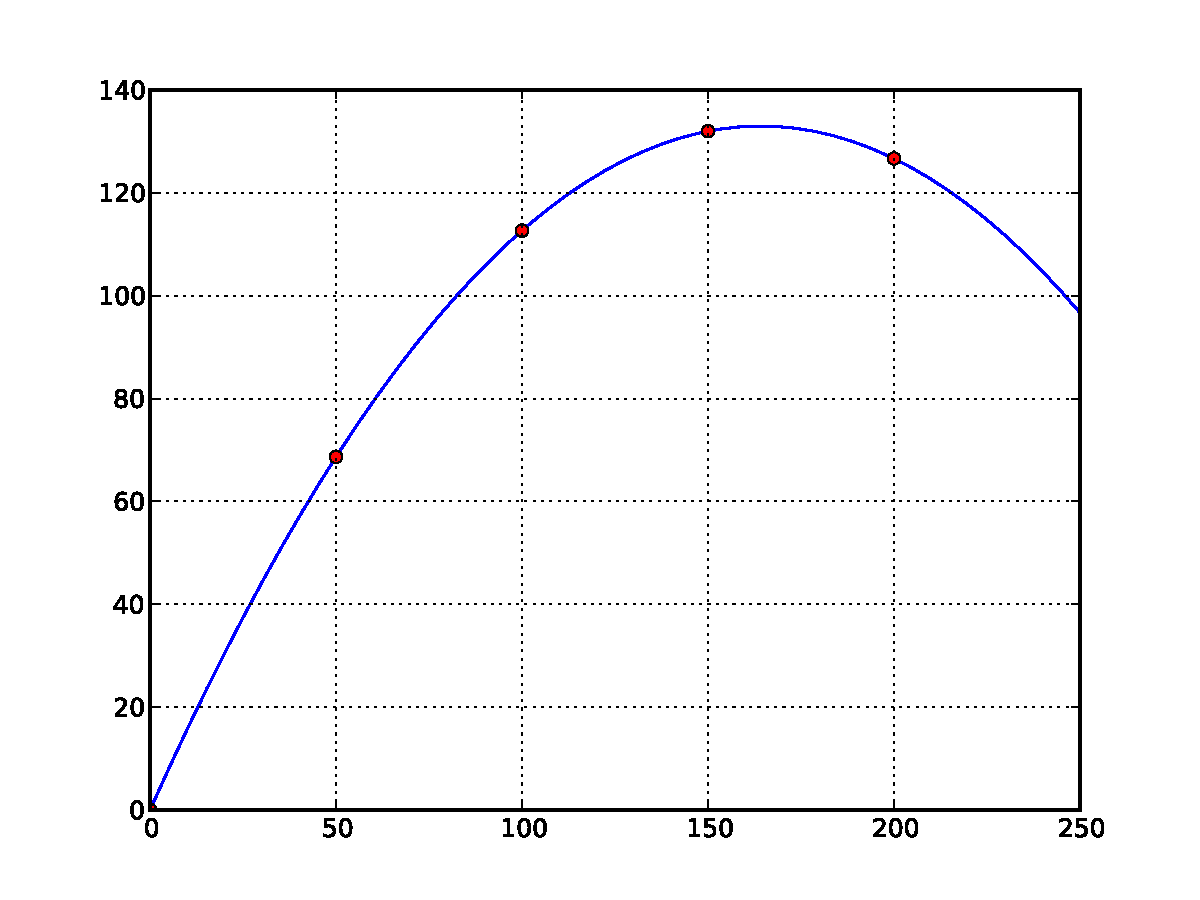
\includegraphics[scale=0.5]{trayectoria1}}%
%\only<2>{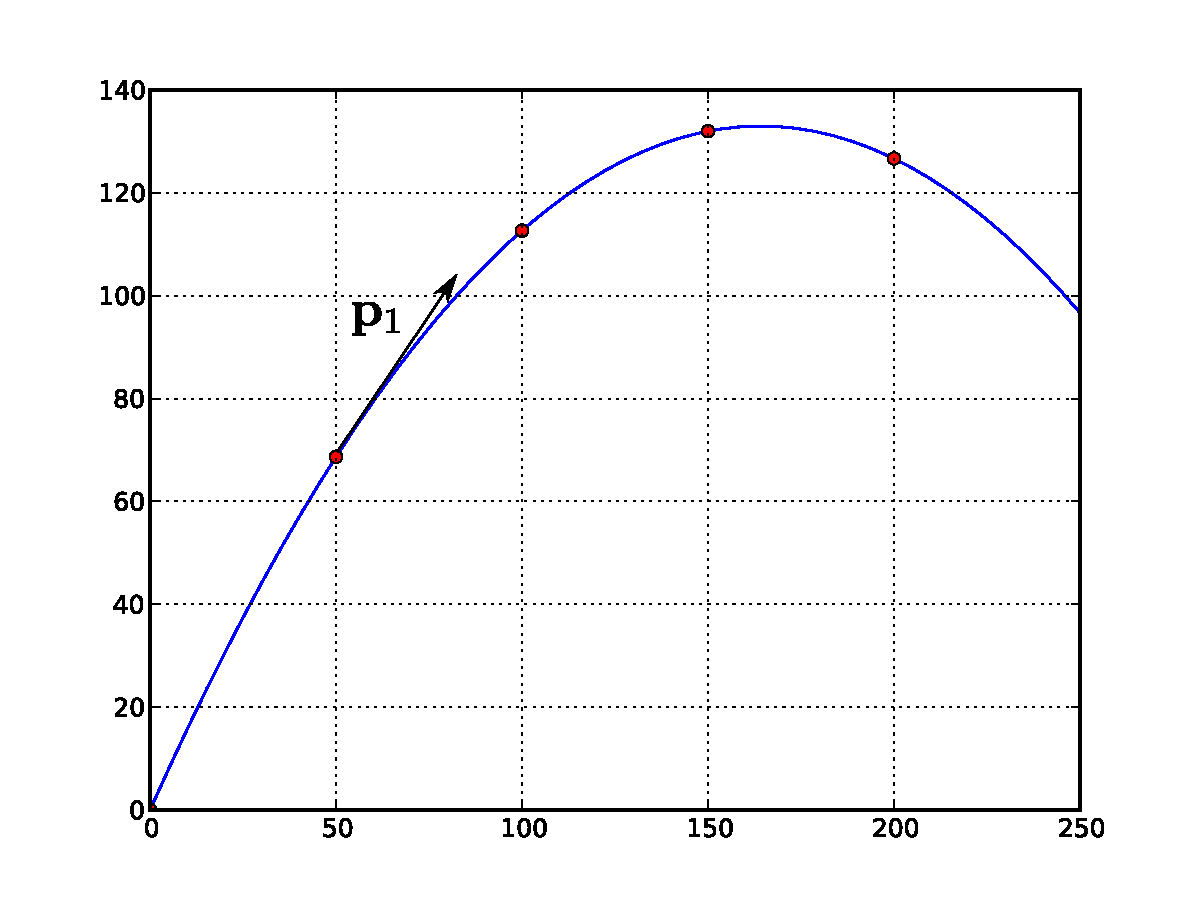
\includegraphics[scale=0.5]{trayectoria2}}%
%\only<3>{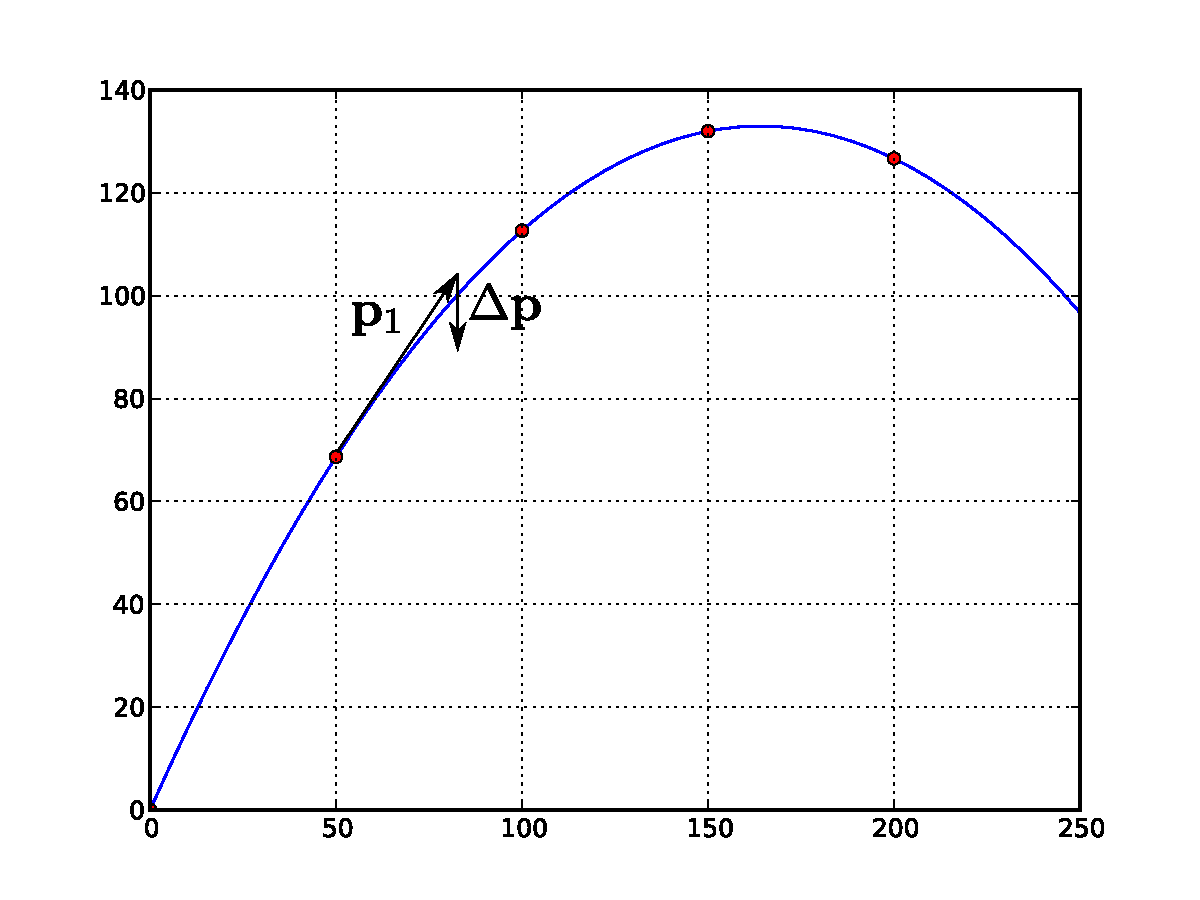
\includegraphics[scale=0.5]{trayectoria3}}%
%\only<4>{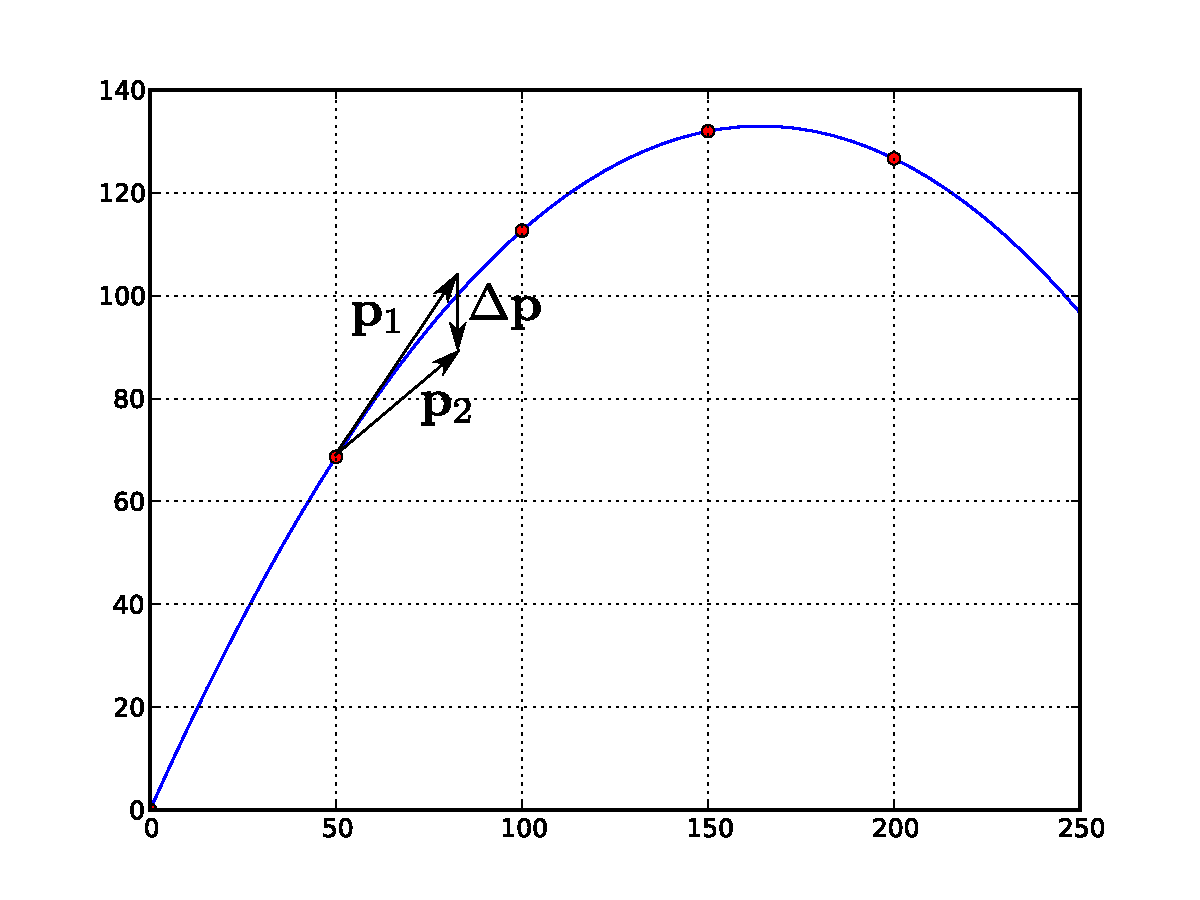
\includegraphics[scale=0.5]{trayectoria4}}%
%\only<5>%
{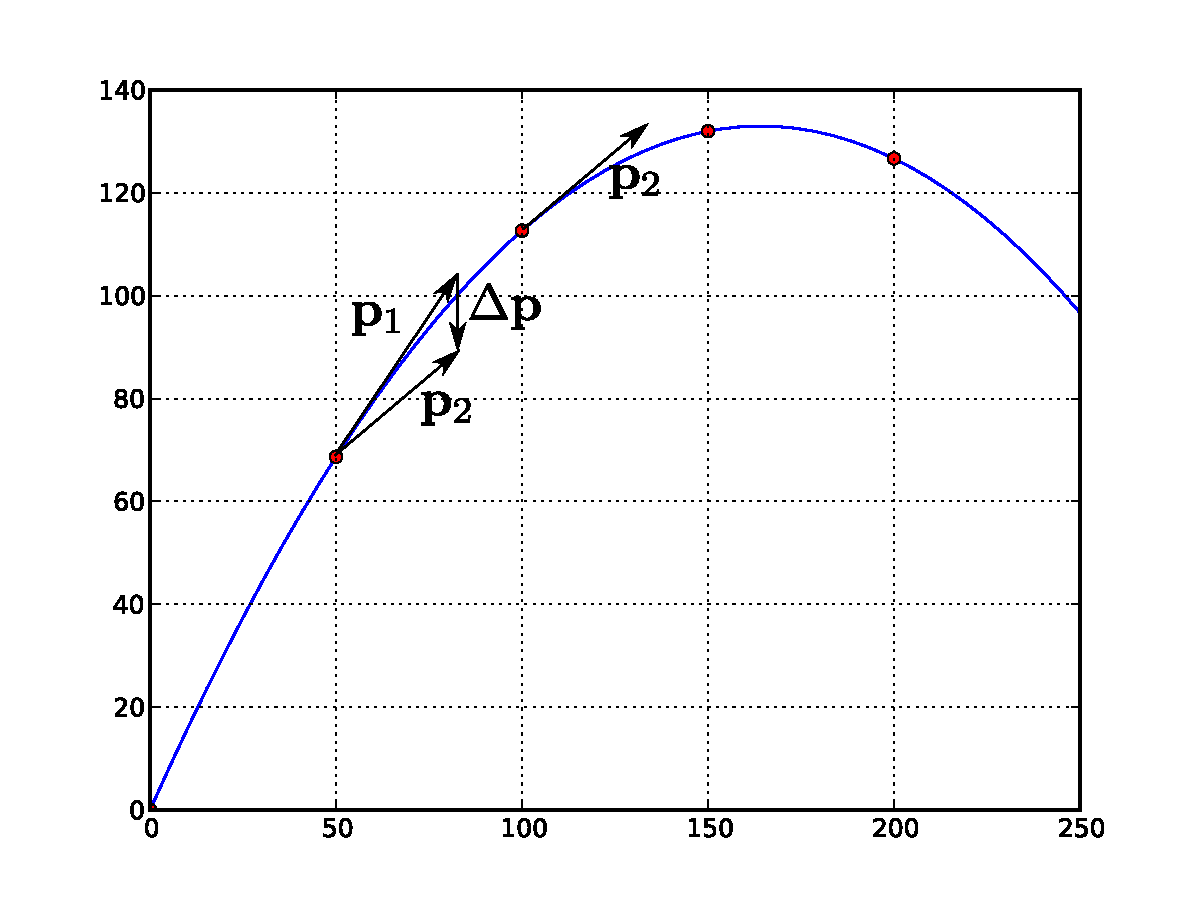
\includegraphics[scale=0.5]{trayectoria5}}
    \caption{Actualización del momentun}
    \label{fig:predtray}
  \end{figure}
\end{frame}

El proceso iterativo que se puede implementar computacionalmente equivale a hacer la integral sobre la ecuación de movimiento dada por el Principio de moméntum. Sin embargo, sólo en casos muy específicos se puede realizar analíticamente la integración de la ecuación de movimiento.

Para ilustrar la integración numérica considere el siguiente programa en \texttt{vpython} de la solución al problema de una partícula de masa $m=0.5\ $Kg, con velocidad inicial $\mathbf{v}_i=(5,0,0)\ $m/s, moviendose bajo la influencia de una fuerza neta gravitacional dada por
\begin{align}
\textbf{F}_{\text{neta}}=&(0,-mg,0)\nonumber\\
=&(0,-4.9,0)\si{\newton}\,,
\end{align}
La implementación con un paso de integración dado por un $\Delta t=\SI{0.01}{\second}$ se ilustra en el siguiente programa:

\begin{frame}[fragile,allowframebreaks]
\begin{lstlisting}
from visual import *
ball=sphere(make_trail=True,pos=vector(-5,5,0),radius=.3, color=color.magenta)
trail=curve(color=(1,1,1))
m=.5
g=9.8
v=vector(5,0,0)
p=m*v
deltat=0.01
Fg=vector(0,-m*g,0)
while True:
    #slow program
    rate(20)
    p=p+Fg*deltat
    ball.pos=ball.pos+(p/m)*deltat
    trail.append(pos=ball.pos)
    if ball.pos[0]>2: raw_input('Stop?')
\end{lstlisting}
\end{frame}

El resultado del programa es la simulación del evento paso a paso hasta alcanzar la posición mostrada en la figura~\ref{fig:CaidaLibreSimple}

\begin{frame}[plain]
  \begin{figure}
    \centering
    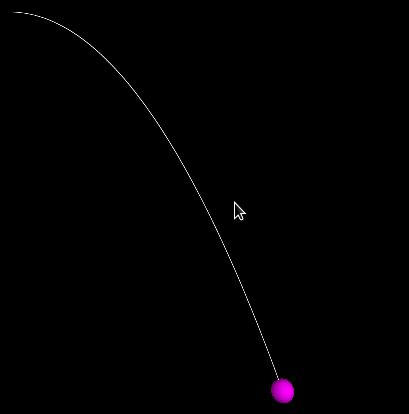
\includegraphics[scale=0.4]{CaidaLibreSimple}
    \caption{Movimiento parabólico integrado numéricamente}
    \label{fig:CaidaLibreSimple}
  \end{figure}
\end{frame}
Tomando el origen de coordenadas en el punto inicial de la bola, podemos obtener las primeras posiciones de la bola repitiendo el proceso manualmente. El resultado de las primeras cinco interacciones se muestra en la Tabla~\ref{tab:caidalibre}
\begin{table}
  \centering
  \begin{tabular}{|c|c|c|}\hline
    $t$ (\si{\second}) & $\mathbf{p}$ (\si{\kilo\gram \meter\per\second}) & $\mathbf{r}$ (\si{\meter})\\\hline
    0.01 & (2.5, -0.049, 0) & (0.05,-0.00098, 0)\\
    0.02 & (2.5, -0.098, 0) & (0.1, -0.00294, 0)\\
    0.03 & (2.5, -0.147, 0) & (0.15,-0.00588, 0)\\
    0.04 & (2.5, -0.196, 0) & (0.2, -0.0098,  0)\\
    0.05 & (2.5, -0.245, 0) & (0.25,-0.0147,  0)\\ 
    $\cdots$ & $\cdots$ & $\cdots$ \\ \hline
  \end{tabular}
  \caption{Primeras cinco posiciones de la bola con respecto al punto inicial}
  \label{tab:caidalibre}
\end{table}



Podemos complicar el programa poniendo rebotes sobre el piso. El programa modificado es
\begin{frame}[fragile,allowframebreaks]
\begin{lstlisting}
from visual import *
ball=sphere(make_trail=True,pos=vector(-5,5,0),radius=.3, color=color.magenta)
floor=box(pos=vector(0,-5,0), size=(12,0.1,12) , color=color.green)
trail=curve(color=(1,1,1))
m=.5
g=9.8
v=vector(0.5,0,0)
p=m*v
deltat=0.01
Fg=vector(0,-m*g,0)
while True:
    #slow programa
    rate(100)
    p=p+Fg*deltat
    ball.pos=ball.pos+(p/m)*deltat
    trail.append(pos=ball.pos)
    if ball.pos.y < floor.pos.y:
        p.y=-p.y

\end{lstlisting}
\end{frame}

\begin{frame}
  El programa genera una animación, de la cual  se ilustra uno de los cuadros en la figura~\ref{fig:caidalibre}
  \begin{figure}
    \centering
    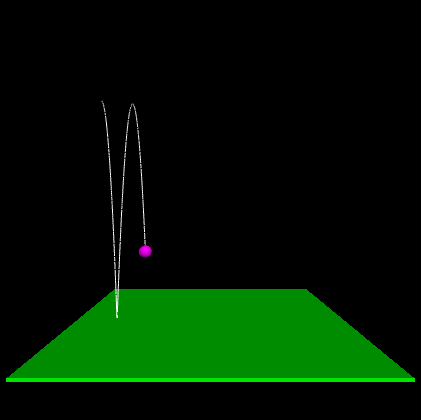
\includegraphics[scale=0.5]{caidalibre}
    \caption{Movimiento parábolico con rebote}
    \label{fig:caidalibre}
  \end{figure}

\end{frame}


Medir la velocidad de un objeto es una tarea familiar, pero ¿cómo
medimos la magnitud de una fuerza?

Una forma simple de medir una fuerza es usar el estiramiento o
compresión de un resorte. 
%Hacer diagrama.
Cuando colgamos un bloque de un resorte, notamos que el resorte se
estira una distancia $s$.  
Si doblamos el peso notamos que el resorte se estira el doble. 
De la misma manera un resorte en posición vertical es comprimido una
distancia $s$ por el mismo bloque, y el doble de la distancia con dos
bloques.

Por consiguiente, podemos usar un resorte para hacer una escala para
medir fuerzas, calibrándolo en términos de cuanta fuerza se necesita
para producir un determinando estiramiento.
 
\subsection{Fuerza de un resorte}

Una ley de fuerza describe matemáticamente como una fuerza depende en una situación. Para un resorte, se ha determinado experimentalmente que la fuerza ejercida por un resorte sobre un objeto pegado al resorte está dada por la siguiente ecuación:
\begin{align}
  \left| \mathbf{F}_{\text{resorte}} \right|=k|\Delta \mathbf{r}|
\end{align}
donde $|\Delta \mathbf{r}|$ es la magnitud del vector desplazamiento entre la posición inicial y final del objeto pegado al resorte, y $k$ es la \emph{constante elástica} del resorte. 

La constante elástica $k$ es un número positivo, y es una propiedad del resorte en particular. Entre más grande $k$ más fuerza se necesita para estirar el resorte. 

Para un resorte moviéndose en una dimensión y con el origen de coordenadas coincidiendo con la posición del objeto cuando el resorte esta relajado, tenemos que la fuerza que el resorte ejerce sobre el objeto cuando se estira una distancia $x$ es
\begin{align}
  \mathbf{F}=-k(x,0,0)
\end{align}


Si consideremos un resorte con un cuerpo pegado a su extremo moviéndose sobre una superficie, debemos considerar la fuerza de fricción entre el cuerpo y la superficie. La Ley que describe esta fuerza fricción $f$, encontrada también por experimentación, es
\begin{align}
  |\mathbf{f}|=\mu m g\,,
\end{align}
donde $\mu$ es el \emph{coeficiente de fricción entre el cuerpo y la superficie}, $m$ es la masa del cuerpo y $g$ es la aceleración gravitacional cerca a la superficie de la Tierra. La dirección de la fuerza de fricción es siempre opuesta a la dirección de movimiento. 

Con está información y con el principio de moméntum podemos simular el movimiento de un cuerpo unido a un resorte sobre una superficie horizontal. La explicación paso a paso del funcionamiento del programa puede encontrarse en este \href{http://nbviewer.ipython.org/urls/raw.github.com/rescolo/spring/master/spring.ipynb}{link}. Mientras el programa definitivo es

\begin{frame}[fragile,allowframebreaks]
\begin{lstlisting}
from __future__ import division
from visual import *


# INITIALIZE WINDOW AND DECLARATIONS

scene.range = vector(1,1,1)
scene.center = vector(0,0,0)
scene.width = 800
scene.height = 600

# CREATE SPRING, WEIGHT AND LABEL OBJECTS

relaxedlength = vector(.60,0,0) # length of spring when it isn't stretched or compressed
spring = helix(pos=(-.75,0,0),axis=relaxedlength, radius=.1,coils=8,thickness=.01,color=color.green)

weight = box(pos=(0,0,0),size=(.3,.3,.3),color=color.yellow)

frictionlessSurface = box(size=(2,.02,.5),pos=(0,-.16,0))
wall = box(size=(.04,.5,.3),pos=(-.77,.1,0),color=color.red)


# SET INITIAL CONDITIONS

spring.constant = 2 # k
weight.mass = 10 # kg
weight.velocity = vector(0,0,0)
weight.acceleration = vector(0,0,0)
weight.force = vector(0,0,0)

#Set the label position
mylabel = label(pos=(0,.4,0))
#spring.displacement
xpos=0.35 
weight.pos=vector(xpos,0,0)
spring.displacement=weight.pos
spring.axis=relaxedlength+spring.displacement
# message to the user
message = "Inititial position:"
message += "\ndisplacement: %.2f" % spring.displacement.x 
mylabel.text = message

\end{lstlisting}
\end{frame}

\subsection{Integración analítica}
Al proceso de evolucionar un sistema a través del tiempo se le llama
integración del movimiento. En algunos caso especiales dicha
integración se puede realizar de forma analítica. El proceso
matemático de integrar una función $f(x)$ en el intervalo $a$, $b$, corresponde a evaluar el área bajo la curva en ese intervalo
\begin{align}
  \int_a^b f(x)\,dx\approx&f(x_0)(x_1-x_0)+f(x_1)(x_2-x_1)+\cdots+f(x_{n-1})(x_n-x_{n-1}) \nonumber\\
\lim_{\Delta x\to 0}\sum_{i=0}^n\,f(x_i)\Delta x_i\,,
\end{align}
donde $f(x_0)=1$, $f(x_{n})=b$ y $\Delta x_i=x_{i+1}-x_i$.

Se puede demostrar que
\begin{align}
  \int_a^b f(x)\,dx=\left. F(x)  \right|_a^b
\end{align}


\begin{table}
  \centering
  \begin{tabular}{lll}
    $f(x)$ & derivada & integral\\
  \end{tabular}
  \caption{Tabla de integrales}
\end{table}

De este modo, por ejemplo, la integral de la función $f(x)=x$ entre $0$ y $a$ es
\begin{align}
  \int_0^a x\,dx=\left.\frac{1}{2}x^2\right|_0^a=\frac{1}{2}a^2\,,
\end{align}
y el área del triángulo correspondiente es
\begin{align}
  \frac{1}{2}\text{base}\times\text{altura}=\frac{1}{2}a^2\,,
\end{align}

Así mismo la integral de una rapidez constante $v$, entre $t_1$ y $t_2$ para un movimiento en línea recta
\begin{align}
  \int_{t_1}^{t_2}v \,dt=v(t_2-t_1)=d=\text{distancia recorrida entre $t_1$ y $t_2$.}
\end{align}
En general, el área de la curva en línea recta de la velocidad en
función del tiempo corresponde a la distancia recorrida. Para el
gráfico de distancia en función del tiempo de la
Fig.~\ref{fig:vinstaprom3}, tendríamos en el plano velocidad en
función del tiempo, una línea recta horizontal entre cero y
$\SI{1}{h}$, una línea recta de $\SI{70}{km/h}$, con área bajo la
curva $\SI{70}{km}$, y otra línea recta entre $\SI{1}{h}$ y
$\SI{2}{h}$ con área $\SI{30}{km}$ para una distancia total recorrida
de $\SI{100}{km}$.

\subsection{Ecuación de movimiento}


Como para un $\Delta t$ infinitesimal, la fuerza siempre se puede considerar constante, el principio de momentum se puede reescribir como
\begin{align}
  \label{eq:28}
  \mathbf{F}_{\text{neta}}=&\lim_{\Delta t\to 0}\frac{\Delta\mathbf{p}}{\Delta t}\nonumber\\
 \mathbf{F}_{\text{neta}}=&\frac{d\mathbf{p} }{dt}
\end{align}
Si $\mathbf{F}_{\text{neta}}$ es conocida, a la ec.~\eqref{eq:28}, se conoce como ecuación de movimiento.

\begin{frame}
  \begin{block}%
{Ecuación de movimiento:}
  \begin{align*}
   \mathbf{F}_{\text{neta}}=&\frac{d\mathbf{p} }{dt}
   \end{align*}
  \end{block}
\end{frame}



\subsection{Caso especial: masa constante}
En el caso especial en que la masa del sistema, $m$, es constante, la ecuación de movimiento puede reescribirse como
\begin{align}
   \mathbf{F}_{\text{neta}}=&\frac{d m\mathbf{v} }{dt}\nonumber\\
   \mathbf{F}_{\text{neta}}=&m\frac{d \mathbf{v} }{dt}\nonumber\\
   \mathbf{F}_{\text{neta}}=&m\mathbf{a}\,.
\end{align}

\begin{frame}
  \begin{block}%
{Caso especial: masa constante}
\begin{align}
   \mathbf{F}_{\text{neta}}=&m\mathbf{a}\,.
\end{align}
\end{block}
\end{frame}

\subsection{Caso especial: Fuerza y masa constante}

Si la fuerza neta es constante en dirección y magnitud en el caso de masa constante, la ecuación de movimiento puede integrarse analíticamente. Para simplificar el análisis consideremos una fuerza neta constante sólo con componente en $x$:
\begin{align}
  \mathbf{F}_{neta}=(F_x,0,0)\,.
\end{align}

La ecuación de movimiento se reduce a
\begin{align}
  a_x=&\frac{F_x}{m}\nonumber\\
\frac{dv_x}{dt}=&\frac{F_x}{m}\nonumber\\
{dv_x}=&\frac{F_x}{m}{dt}\,.
\end{align}
Integrando a ambos lados de la igualdad, desde un tiempo inicial $t_i$ a un tiempo final $t$, con $v_{xi}=v_x(t_i)$ y $v_x=v_x(t)$, tenemos
\begin{align}
  \int_{v_{xi}}^{v_x} d v_x =&\int_{t_i}^t \frac{F_x}{m}{dt}\nonumber\\
  v_x-v_{xi} =&\frac{F_x}{m}\int_{t_i}^t {dt}\,
\end{align}
y despejando en términos de la velocidad final
\begin{align}
  \label{eq:36}
  v_x =&v_{xi}+\frac{F_x}{m}(t-t_i)\nonumber\\
=&v_{xi}+\frac{F_x}{m}\Delta t\,.
\end{align}
Integrando de nuevo
\begin{align}
  \frac{dx}{dt} =&v_{xi}+\frac{F_x}{m}(t-t_i)\nonumber\\
  {dx} =&v_{xi}{dt}+\frac{F_x}{m}(t-t_i){dt}\,,
\end{align}
e integrando de nuevo con $x_i=x(t_i)$ y $x=x(t)$, tenemos
\begin{align}
  \int_{x_i}^{x}{dx} =&v_{xi}\int_{t_i}^t{dt}+\frac{F_x}{m}\int_{t_i}^t{dt}(t-t_i){dt}\,.
\end{align}
Haciendo $u=t-t_i$, $du=dt$, obtenemos
\begin{align}
\int(t-t_i)dt=\int u du=\frac{1}{2}u^2=\frac{1}{2}(t-t_i)^2\,,
\end{align}
de modo que
\begin{align}
  x-x_i=&v_{xi}(t-t_i)+\frac{F_x}{m}\left.\frac{1}{2}(t-t_i)^2\right|^t_{t_i}
\end{align}
\begin{align}
  x=&x_i+v_{xi}(t-t_i)+\frac{1}{2}\frac{F_x}{m}
  \left[
    (t-t_i)^2-(t_i-t_i)^2
  \right]\nonumber\\
  x=&x_i+v_{xi}(t-t_i)+\frac{1}{2}\frac{F_x}{m}(t-t_i)^2
\end{align}
\begin{frame}
  \begin{block}%
{Solución analítica:} al problema de movimiento en una dimensión bajo la influencia de una fuerza constante
\begin{align}
   x=&x_i+v_{xi}(t-t_i)+\frac{1}{2}\frac{F_x}{m}(t-t_i)^2\nonumber\\
   =&x_i+v_{xi}\Delta t+\frac{1}{2}\frac{F_x}{m}\Delta t^2\,.
\end{align}
  \end{block}
\end{frame}

Si eliminamos $\Delta t$, usando la ec.\eqref{eq:36}, tenemos
\begin{align*}
  x=&x_i +v_{xi}(v_x-v_{xi})\frac{m}{F_x}+\frac{1}{2}\frac{F_x}{m}(v_x-v_{xi})^2\frac{m^2}{F_x^2}\nonumber\\
  x=&x_i +(v_{xi}v_x-v_{xi}^2)\frac{m}{F_x}+\frac{1}{2}(v_x^2-2 v_x v_{xi}+v_{ix}^2)\frac{m}{F_x}\nonumber\\
x=&x_i +\frac{1}{2}(v_x^2-v_{ix}^2)\frac{m}{F_x}\,.
\end{align*}
Reorganizando términos tenemos
\begin{align}
  \label{eq:tray0}
  v_x^2-v_{ix}^2=-2\frac{F_x}{m}(x-x_i)\,.
\end{align}


Un ejemplo de fuerza constante, es la fuerza gravitacional sobre un objeto de masa $m$ que se encuentra cerca a la superficie de la tierra:
\begin{align}
  \label{eq:29}
  \mathbf{F}_{\text{grav}}=(0,F_y,0)\approx(0,-mg,0).
\end{align}
El signo menos índica que la fuerza va dirigida hacía la superficie de la tierra, donde hemos establecido el origen de coordenadas

Si dicho cuerpo cae libremente desde una altura $y_i$ desde la superificie de la tierra, y con una velocidad $v_{yi}$, la ecuación para su altura $y$ desde un origen de coordenadas sobre la superficie de la tierra es
\begin{align}
\label{eq:31}
   y=&y_i+v_{yi}(t-t_i)+\frac{1}{2}\frac{F_y}{m}(t-t_i)^2\nonumber\\
   y=&y_i+v_{yi}(t-t_i)-\frac{1}{2}g(t-t_i)^2\,.
\end{align}
mientras que para la componente de la velocidad en $y$, tenemos de la ec.~\eqref{eq:36}
\begin{align}
  \label{eq:37}
    v_y =&v_{yi}-g(t-t_i)\,,
\end{align}

\begin{frame}
  \begin{block}%
{Solución analítica:} al problema de caida libre en la dirección $y$ perpendicular a la superficie de la tierra y con origen de coordenadas sobre la superficie de la tierra:
\begin{align*}
     y=&y_i+v_{yi}(t-t_i)-\frac{1}{2}g(t-t_i)^2\nonumber\\
     v_y =&v_{yi}-g(t-t_i)\nonumber\\
     a_y=&-g\,.
\end{align*}

  \end{block}
\end{frame}


\subsection{Ecuación de la trayectoria}
Para un cuerpo en movimiento vertical bajo la influencia de una fuerza gravitacional constante, tenemos que si la rapidez inicial es $v_0$ para una altura inicial $y_0$, entoces de \eqref{eq:37}
\begin{align}
  \Delta t=\frac{v_0-v}{g}
\end{align}
sustituyendo en ec.~\eqref{eq:caidalibre}
\begin{align}
  y-y_0=&v_0(v_0-v)/g-\tfrac{1}{2}g(v_0-v)^2/g^2\nonumber\\
       =&v_0^2/g-vv_0/g-\tfrac{1}{2}(v_0^2/g-2vv_0/g+v^2/g)\nonumber\\
       =&\tfrac{1}{2}v_0^2/g-\tfrac{1}{2}v_0^2/g\nonumber\\
       =&\tfrac{1}{2}(v_0^2-v^2)/g\,,
\end{align}
de donde obtenemos la ecuación de la trayectoria (vec eq.~(\ref{eq:tray0}):
\begin{align}
  \label{eq:trayectoriay}
  v^2-v_0^2=-2g(y-y_0)\,,
\end{align}
Esta \'ultima ecuaci\'on esta relacionada con la conservaci\'on de energ\'\i a cin\'etica m\'as energ\'\i a potencia, como se definir\'a luego.


\subsection{Conservación de momentum}
Volviendo al problema general, de la ec.~\eqref{eq:28} podemos ver que si el momentum es constante (en dirección, magnitud y masa)
\begin{align}
  \mathbf{F}_{\text{neta}}=&\frac{d\mathbf{p}}{dt}\nonumber\\
=&0\,.
\end{align}
En otras palabras:
\begin{frame}
  \begin{block}%
{Ley de Conservación de Moméntum:} \textbf{Si la fuerza neta actuando sobre un sistema es cero, el momentum total del sistema es constante}
  \end{block}
\end{frame}

En componentes:
\begin{align}
  F_{\text{neta},x}=&\frac{d p_x}{dt}\nonumber\\
  F_{\text{neta},y}=&\frac{d p_y}{dt}\nonumber\\
  F_{\text{neta},z}=&\frac{d p_z}{dt}\,,
\end{align}
y podemos ver que si alguna dirección del moméntum es constante, entonces la fuerza neta en esa dirección es cero, y viceverza. 

De acuerdo al teorema de Noether debe existir una simetría asociada a
la conservación de cada una de la direcciones del moméntum. 
La simetría correspondiente es la homogeneidad del espacio en cada una
de sus tres direcciones independientes.
Esta simetría se refleja en el hecho de que si realizamos un
experimento en un sitio determinado y luego lo repetimos en el
laboratorio de al lado, del frente, o del piso superior, debemos
obtener exactamente el mismo resultado. 
La regla de transformación correspondiente es que las leyes de la física deben ser invariante bajo el cambio, por ejemplo
\begin{align*}
  x\to x'=x+a\,,
\end{align*}
con $a$ constante.
En efecto
\begin{align*}
  F'_{\text{neta},x}=&\frac{dp'_{x}}{dt}\nonumber\\
=&m\frac{dv'_{x}}{dt}\nonumber\\
=&m\frac{d}{dt}\frac{dx'}{dt}\nonumber\\
=&m\frac{d}{dt}\frac{d(x+a)}{dt}\nonumber\\
=&m\frac{d}{dt}\frac{d(x)}{dt}\nonumber\\
=&m\frac{dv_{x}}{dt}\nonumber\\
=&\frac{dp_{x}}{dt}=F_{\text{neta},x}\,,
\end{align*}
de modo que dos observadores en dos laboratorios separados por una
distancia $x'=x+a$, deben medir la misma cantidad de movimiento para
el movimiento de un cuerpo sometido a una fuerza $F_{\text{neta},x}$.



En el caso de la fuerza gravitacional, si despreciamos la resistencia del aire, de la ec.~\eqref{eq:29} podemos ver que que la fuerza neta en $x$ y en $z$ es cero. Por lo tanto el momentum inicial en la dirección $x$ y $z$ se debe conservar. 

Supongamos que un cuerpo se mueve bajo la influencia de la fuerza gravitacional en un planeta sin atmosfera con aceleración gravitacional $g$. Por simplicidad, escojamos como $x$ la dirección inicial del cuerpo paralela a la superficie del planeta. Dicha dirección se debe mantener constante, de modo que
\begin{align*}
  \frac{d p_x}{dt}=&0\nonumber\\
  m\frac{d v_x}{dt}=&0\nonumber\\
  \frac{d v_x}{dt}=&0\nonumber\\
  {d v_x}=&0\nonumber\\
  \int_{v_{xi}}^{v_x}{d v_x}=&0\nonumber\\
  v_x-v_{xi}&=0\nonumber\\
  v_x=&v_{xi}\,.
\end{align*}
integrando de nuevo
\begin{align}
  \frac{dx}{dt}=&v_{xi}\nonumber\\
  dx=&v_{xi}{dt}\nonumber\\
  \int_{x_i}^x dx=&v_{xi}\int_{t_i}^t{dt}\nonumber\\
  x-x_i=&v_{xi}(t-t_i)\,.
\end{align}
y recuperamos la
\begin{frame}
  \begin{block}%
{solución analítica:} al problema del movimiento en una dimensión en ausencia de fuerzas externas
\begin{align}
  \label{eq:30}
  x=&x_i+v_{xi}(t-t_i)\,.
\end{align}
  \end{block}
\end{frame}

Combinado las ecuaciones \eqref{eq:30} y \eqref{eq:31} obtenemos la
\begin{frame}
  \begin{block}%
{solución analítica:} al problema de movimiento parábolico despreciando la resistencia del aire
\begin{align}
  \label{eq:32}
  x=&x_i+v_{xi}(t-t_i)=x_i+v_{xi}\Delta t\nonumber\\
  y=&y_i+v_{yi}(t-t_i)-\frac{1}{2}g(t-t_i)^2=y_i+v_{yi}\Delta t-\frac{1}{2}g\Delta t^2\,.
\end{align}
El vector de desplazamiento es
\begin{align}
\mathbf{r}=(x,y,0)
\end{align}
%hacer diagrama
Derivando con respecto al tiempo obtenemos las velocidades (ver ec.~\eqref{eq:37})
\begin{align}
  \label{eq:33}
  v_x=\frac{dx}{dt}=&v_{xi}&\text{velocidad constante}\nonumber\\
  v_y=\frac{dy}{dt}=&v_{yi}-\frac{1}{2}g(2(t-t_i))&\nonumber\\
  =&v_{yi}-g(t-t_i)&\text{aceleración constante}\,,
\end{align}

  \end{block}
\end{frame}



\begin{itemize}
\item[\textbf{Ejemplo:}] \textbf{Una bola con resistencia de aire despreciable (2D, Fuerza constante):}
Una bola de masa 500~g está inicialmente en el suelo, en una ubicación $(0,0,0)\ $m. La bola es entonces pateada con una velocidad inicial $(3,7,0)\ $m/s.
\begin{enumerate}
\item ¿Donde estará la bola medio segundo después?
\label{item:8}
\item ¿En que tiempo la bola golpeará el piso?
\label{item:9}
\end{enumerate}
Haga la aproximación que la resistencia del aire es despreciable.


\item[\textbf{Solución:}] Sistema: bola\\
Entorno: Tierra\\
Diagrama de cuerpo libre: ver figura\\
Tiempo inicial: El instante en que el pie ya no esta en contacto con la bola
\begin{itemize}
\item[~\ref{item:8}]
Después de medio segundo, y como se ilustra en la figura~\ref{fig:parabgraph1}
\begin{align}
  x_f=&x_i+v_{xi}\Delta t\nonumber\\
  =&0+(3\ \text{m/s})(0.5\ \text{s})=1.5\ \text{m}
\end{align}
Para el movimiento en $y$ tenemos
\begin{align}
  y_f=&y_i+v_{yi}\Delta t-\frac{1}{2}g \Delta t^2\nonumber\\
=& 0+(7\ \text{m/s})(0.5\ \text{s})-\frac{1}{2}(9.8\ \text{N/kg})(0.5\ \text{s})^2=2.275\ \text{m}
\end{align}
El vector final de desplazamiento después de $\SI{0.5}{\second}$ es
\begin{align}
  \mathbf{r}_f=(1.5,2.75,0)\ \text{m}
\end{align}
Comprobación: Las unidades son correctas, y la bola se ha movido en la dirección apropiada
\item[~\ref{item:9}] Tiempo final: El instante justo antes de que la bola golpee el piso. En ese instante sabemos que $y_f=0$, de modo que podemos encontrar $\Delta t$
  \begin{align*}
    0=0+v_{yi}\Delta t-\frac{1}{2}g\Delta t^2
  \end{align*}
  \begin{align*}
 \Delta t(v_{yi}-\frac{1}{2}g\Delta t)=0   
  \end{align*}
con soluciones
  \begin{align}
    \Delta t=&0 &\text{o}\qquad v_{yi}-\frac{1}{2}g\Delta t=&0
  \end{align}
El segundo valor es el tiempo cuando la bola retorna al suelo
\begin{align}
  \Delta t=&\frac{2 v_{yi}}{g}\nonumber\\
=&\frac{2(\SI{7}{m/s})}{\SI{9.8}{\newton\per\kilo\gram}} =\SI{1.43}\ \text{s}
\end{align}
El movimiento en $y$ es ilustrado en la figura~\ref{fig:parabgraph3}, mientras que la trayectoria real es ilustrada en la figura~\ref{fig:parabgraph5}.
\end{itemize}

\end{itemize}



\begin{frame}
\begin{figure}
  \centering
  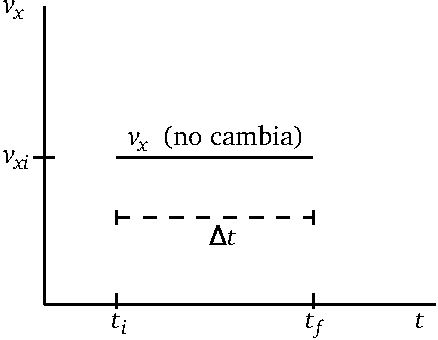
\includegraphics[scale=0.9]{parabgraph1} 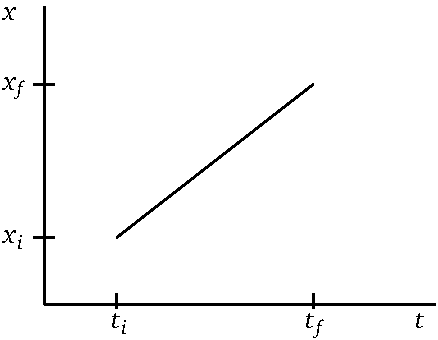
\includegraphics[scale=0.9]{parabgraph2}
  \caption{Movimiento de la bola en $x$}
  \label{fig:parabgraph1}
\end{figure}
\end{frame}

\begin{frame}
\begin{figure}
  \centering
  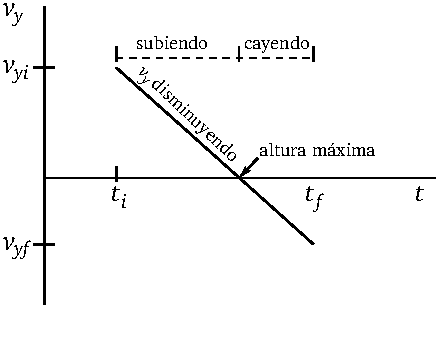
\includegraphics[scale=0.9]{parabgraph3}  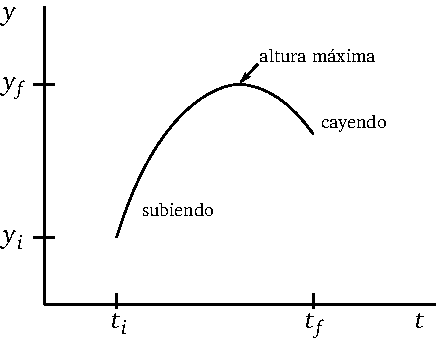
\includegraphics[scale=0.9]{parabgraph4}
  \caption{Movimiento de la bola en $y$}
  \label{fig:parabgraph3}
\end{figure}
\end{frame}

\begin{frame}
\begin{figure}
  \centering
  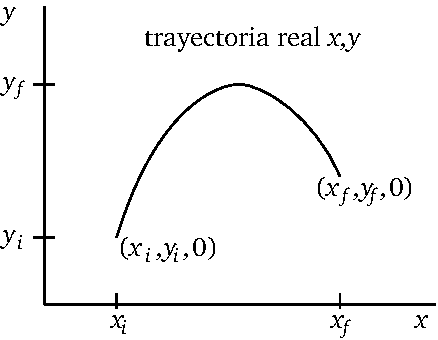
\includegraphics{parabgraph5}
  \caption{Movimiento de la bola en el plano $x-y$}
  \label{fig:parabgraph5}
\end{figure}
\end{frame}

\subsection{Ejemplos movimiento parabólico}

\begin{inprogress}
  Ejemplo notas Kowalski 3-13
\end{inprogress}

\begin{itemize}
\item[\textbf{Ejemplo:}] Una piedra es lanzada hacia arriba desde lo alto de un edificio con una velocidad inicial de 20 m/s directamente hacia arriba. El edificio tiene 50 m de alto, y la piedra falla en golpear el edificio en su camino hacia abajo.
  \begin{enumerate}
  \item \textquestiondown Qu\'e tiempo le toma a la piedra alcanzar su m\'axima altura?
    \begin{align}
      v(t)=v_0-gt\,.
    \end{align}
    A la altura m\'axima $v=0$, y con $v_0=+20$ m/s
    \begin{align}
      t_{\text{max}}=&\frac{v_0}{g}\nonumber\\
      =&\frac{20}{9.8}\ s\nonumber\\
      \approx&2.04\ s
    \end{align}
  \item \textquestiondown Cual es la m\'axima altura desde la base del edificio?:\\
    Tomando el origen de coordenadas en la base del edificio:
    \begin{align}
      y_{\text{max}}=&y_0+v_o t-\frac{1}{2}g t^2\nonumber\\
      \approx&50+20\timesm2.04-\tfrac{1}{2}\timesm9.8\timesm(2.04)^2\nonumber\\
      \approx&70.4\ \text{m}\,,
    \end{align}
  \item \textquestiondown Cual es el tiempo necesario para que la piedra retorne al nivel de la torre?\\
    \begin{align}
      t_{\text{torre}}=2t_{\text{max}}\approx4.08\ \text{s}\,.
    \end{align}
  \item \textquestiondown La velocidad a ese instante?\\
    \begin{align}
      v=&v_0-gt\nonumber\\
      \approx&20-9.8\timesm4.08\\
      v_{\text{torre}}\approx&-20\ \text{m/s}\,,
    \end{align}
    La misma magnitud que la velocidad inicial pero con direcci\'on opuesta. La velocidad incial estar\'\i a representada por un vector $\mathbf{v}_0$: $\uparrow$, mientras que $\mathbf{v}_{\text{torre}}:$ $\downarrow$.
  \item \textquestiondown Cual es la velocidad y posici\'on (desde la base del edificio) despu\'es de $t=5\ \text{s}$?
    \begin{align}
      v(5)\approx 20-9.8\timesm5\approx-29.0\ \text{s}\,.
    \end{align}
    \begin{align}
      y(5)\approx50+20\timesm5-\tfrac{1}{2}\timesm9.8\timesm5^2\approx27.5\ \text{m}\,.
    \end{align}
  \item \textquestiondown Cual es la velocidad y el tiempo cuando la piedra golpea el piso?
    \begin{align}
      y_0=&50\ \text{m} & y_{\text{final}}=0\nonumber\\
      \mathbf{v}_0=&20\hat{\mathbf{j}}\ \text{m/s} & \\
    \end{align}

    \begin{align}
      v^2=&v_0^2-2g(y_{\text{final}}-y_0)\nonumber\\
      =&v_0^2-2g(0-y_0)\nonumber\\
      \approx&20^2+2\timesm9.8\timesm 50\,,
    \end{align}
de donde
\begin{align}
  \mathbf{v}_{\text{final}}=-37.1 \hat{\mathbf{j}}\ \text{m/s}\,.
\end{align}
\begin{align}
  t_{\text{final}}=&(v_0-v_{\text{final}})/g\nonumber\\
  \approx&(20+37.1)/9.8\approx5.83\,s
\end{align}
  \end{enumerate}
\end{itemize}

\subsection{Movimiento parabólico completo}

En un movimiento parabólico completo, donde un cuerpo es lanzado desde
el suelo con cierta velocidad inicial y retorna al suelo sobre una
superficie horizontal, podemos especificar el alcance $R$ y la altura
máxima $y_{\text{max}}$ en términos de la rapidez inicial, $v$, y el
ángulo de lanzamiento $\theta$. Como
$\mathbf{r}_i=(x_i,y_i,0)=(0,0,0)$, tenemos
  \begin{enumerate}
  \item Altura máxima: se obtiene de la condición $v_y=0$. Reemplazando en la ec.~\eqref{eq:33}
    \begin{align}
      0=v_{yi}-g\Delta t\,,
    \end{align}
de modo que para alcanzar $y_{\text{max}}$ el cuerpo se tarda
\begin{align}
  \label{eq:34}
  \Delta t=\frac{v_{yi}}{g}\,.
\end{align}
Reemplazando \eqref{eq:34} en \eqref{eq:32}, tenemos
\begin{align}
  y_{\text{max}}=&v_{yi}\frac{v_{yi}}{g}-\frac{1}{2}g\frac{v_{yi}^2}{g^2}\nonumber\\
  =&\frac{v_{yi}^2}{g}-\frac{1}{2}\frac{v_{yi}^2}{g}\nonumber\\
  =&\frac{1}{2}\frac{v_{yi}^2}{g}\,.
\end{align}
En términos de la rapidez inicial y el ángulo de lanzamiento tenemos
\begin{align}
  y_{\text{max}}=\frac{v^2_i}{g}\sin^2\theta\,,
\end{align}
La mayor de las alturas máximas se obtiene para $\theta=\pi/2=90^\circ$, es decir cuando la velocidad inicial está toda en $y$.
\item Alcance: se obtiene de la condición: $y=0$. Reemplazando en la ec.~\eqref{eq:32}
  \begin{align}
    0=&v_{yi}\Delta t-\frac{1}{2}g\Delta t^2\nonumber\\
    =&\Delta t(v_{yi}-\frac{1}{2}g\Delta t)\to
    \begin{cases}
      \Delta t=0 & x=0\\
      v_{yi}-\frac{1}{2}g\Delta t=0 & x=R\\
    \end{cases}
\,,
  \end{align}
de modo que para alcanzar $R$ el cuerpo se tarda
\begin{align}
 \label{eq:35}
  \Delta t=\frac{2v_{yi}}{g}\,.
\end{align}
Reemplazando \eqref{eq:35} en \eqref{eq:32}, tenemos
\begin{align}
  R=&v_{xi}\frac{2v_{yi}}{g}\nonumber\\
  =&\frac{2v_{xi}v_{yi}}{g}\,.
\end{align}
En términos de la rapidez inicial y el ángulo de lanzamiento tenemos
\begin{align}
  R=&\frac{2v^2_i}{g}\cos\theta\sin\theta\,,
\end{align}
y usando
\begin{align}
  \sin(\alpha+\beta)=\sin\alpha\sin\beta+\cos\alpha\sin\beta
\end{align}
tenemos que $\sin(2\theta)=2\sin\theta\cos\theta$, y
\begin{align}
  R=\frac{v_0^2}{g}\sin(2\theta)\,,
\end{align}
de modo que el alcance máximo se obtiene para $\theta=\pi/4=45^\circ$,
es decir, cuando las componentes de la velocidad inicial se reparten
por igual en $x$ y $y$.
  \end{enumerate}



\begin{inprogress}
  Copiar ejemplo de tanque en movimiento disparando verticalmente hacia arriba.
\end{inprogress}

\begin{itemize}
\item[\textbf{Ejemplo}] \textbf{El mono}\\
Un mono se suelta de un \'arbol a una altura $h_0$ en el mismo instante en el que le disparan. \textquestiondown Con que \'angulo se debe apuntar al mono para atinarle?
  \begin{align}
    y_{\text{bala}}(t)=&(v_0\sin\alpha)t-\tfrac{1}{2}g t^2\nonumber\\
    y_{\text{mono}}(t)=&h_0-\tfrac{1}{2}g t^2\,.
  \end{align}
Supongamos que en el punto $P$: $y_{\text{bala}}=y_{\text{mono}}$. Entonces
\begin{align}
  v_0 t_P\sin\alpha=&h_0\,.
\end{align}
Sea $D$ la distancia horizontal recorrida en el tiempo $t_P$. Como $v_x=v_0\cos\alpha=\text{cte}$, entonces
\begin{align}
  (t_Pv_0\cos\alpha)\frac{\sin\alpha}{\cos\alpha}=h_0\,,
\end{align}
de modo que
\begin{align}
  \tan\alpha=\frac{h_0}{D}\,.
\end{align}
Entonces, para atinarle al mono, se debe apuntar directamente a \'el.

\item[\textbf{Ejercicio}]Calcula la m\'\i nima distancia para que una bala disparada con una velocidad de $3\ \text{m/s}$, apuntada a la cabeza de un mono de $0.5\ $m de altura y a $10\ $m del suelo y que se quede quieto, pase justo por debajo de sus pies. (Respuesta: $95.3\ $m)
\end{itemize}





\begin{borrar}
En una dimensi\'on es establecida por la ecuaci\'on
\begin{align}
  \label{eq:2ndlaw1d}
  a=\frac{F}{m}\,,
\end{align}
donde $F$ es la fuerza actuando sobre un cuerpo de masa $m$. 

\begin{itemize}
\item[\textbf{Ejemplo:}] Establezca cual es la fuerza asociada a la ca\'\i da libre.

Para obtener la ecuaci\'on de movimiento:
\begin{align}
  \frac{d^2y(t)}{dt^2}=-g\,,
\end{align}
se requiere que un cuerpo en ca\'\i da libre de masa $m$ sufra una fuerza:
\begin{align}
  F=-m\,g\,.
\end{align}

\end{itemize}

En general, la ecuaci\'on de movimiento en una dimensi\'on puede escribirse como
\begin{align}
  \frac{d^2x(t)}{dt^2}-\frac{F(x)}{m}=0\,.
\end{align}

La ecuaci\'on~(\ref{eq:2ndlaw1d}) puede escribirse en una forma m\'as familiar como
\begin{align}
  F=m\,a\,.
\end{align}
En el sistema internacional de unidadades (SI), la unidad de Fuerza es el \emph{Newton} (N), la unidad de masa es el \emph{Kilogramo} (kg), y la aceleraci\'on es en metros por segundo al cuadrado ($\metre\per\second\squared$):
\begin{align}
  F=&m\,a\nonumber\\
&[\kilo\gram]
\left[\frac{\meter}{\second\squared}\right]\nonumber\\
=&\newton\,.
\end{align}
La masa es la resistencia de un cuerpo a cambiar su estado de movimiento.

En t\'erminos vectoriales, concluimos que la fuerza total $\mathbf{F}$ en un cuerpo de masa $m$ es
\begin{align}
  \mathbf{F}=\sum_i \mathbf{F}_i\,.
\end{align}
Si $\mathbf{a}$ es la aceleraci\'on neta, y $\mathbf{a}_i$ la aceleraci\'on debida a $\mathbf{F}_i$ solamente, entonces tenemos
\begin{align}
  \mathbf{F}=&\sum_i \mathbf{F}_i\nonumber\\
  =&\sum_i m\mathbf{a}_i\nonumber\\
  =&m\sum_i \mathbf{a}_i\nonumber\\
  =&m\mathbf{a}\,,
\end{align}
o
\begin{align}
  \label{eq:fma}
  \mathbf{F}=m\mathbf{a}\,.
\end{align}
Esta es la segunda Ley de movimiento de Newton. Las fuerzas surgen de las \emph{interacciones} entre dos sistemas. Por esto raz\'on, en cuanto aislemos un cuerpo lo suficiente de sus alrededores, esperaremos que el cuerpo se mueva uniformemente en un sistema inercial.

Cuando se define cuerpo aislado, el aislamiento significa eliminar las interacciones. Usualmente, para aislar un cuerpo es suficiente moverlo lo suficientemente lejos de todo lo dem\'as. En tal caso las interacciones pueden reducirse tanto como uno desee.
  
\end{borrar}


\begin{itemize}
\item[\textbf{Ejemplo}:] Para el diagrama en la figura~\ref{fig:forces}, calcule la fuerza resultante.
  \begin{figure}
    \centering
    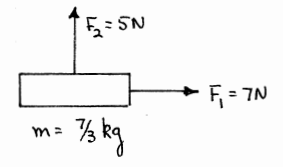
\includegraphics[scale=0.7]{forces}
    \caption{Fuerza resultante}
    \label{fig:forces}
  \end{figure}

Se escoge un sistema de coordenadas tal que
\begin{align}
  \mathbf{F}_1=&7\hat{\mathbf{i}}+0\hat{\mathbf{j}}\nonumber\\
  \mathbf{F}_2=&0\hat{\mathbf{i}}+5\hat{\mathbf{j}}\,.
\end{align}
Entonces
\begin{align}
  \mathbf{F}_R=\mathbf{F}_1+\mathbf{F}_2=
  7\hat{\mathbf{i}}+5\hat{\mathbf{j}}\,.
\end{align}
La aceleraci\'on, que esta en la misma direcci\'on que la fuerza esta dada por
\begin{align}
  \mathbf{a}=\frac{\mathbf{F}_R}{m}=\frac{7\hat{\mathbf{i}}+5\hat{\mathbf{j}}}{7/3}=3\hat{\mathbf{i}}+\frac{15}{7}\hat{\mathbf{j}}\,.
\end{align}

\item[\textbf{Ejemplo:}] Un disco plano de masa $m=\SI{2}{\kilo\gram}$, se desliza sobre un lago congelado con una rapidez inicial de $v=\SI{5}{\meter\per\second}$. La fuerza de fricci\'on tiene un valor constante de $f=\SI{4}{\newton}$ opuesta al movimiento. \textquestiondown cuan lejos avanza el disco antes de detenerse?

Escogiendo apropiadamente el sistema de coordenadas, tenemos:
\begin{align}
  -f \hat{\mathbf{i}}=m\mathbf{a}\,,
\end{align}
de donde
\begin{align}
  \mathbf{a}=-\frac{f}{m}\hat{\mathbf{i}}=\frac{-\SI{4}{\newton}}{\SI{2}{\kilo\gram}}\hat{\mathbf{i}}={-2\hat{\mathbf{i}}}{\si{\meter\per\second\squared}}\,.
\end{align}
De la cinemática del problema tenemos (eq.~\eqref{eq:trayectoriay})
\begin{align}
  v_f^2-v_0^2=2 a x\,.
\end{align}
Cuando el disco se detiene $\mathbf{v}_f=0$, de modo que
\begin{align}
  -v_0^2=&2ax\nonumber\\
  x=&-\frac{v_0^2}{2a}=\SI{6.25}{\meter}\,.
\end{align}


\end{itemize}

\subsection{Tercera Ley de Newton}
Las fuerzas siempre aparecen en pares: si un cuerpo $b$ ejerce una fuerza $\mathbf{F}_a$ en un cuerpo $a$, entonces debe haber otra fuerza $\mathbf{F}_b$ actuando en el cuerpo $b$, debido al cuerpo $a$, tal que
\begin{align}
  \mathbf{F}_b=-\mathbf{F}_a\,.
\end{align}
En otras palabras
\begin{align}
  \text{acci\'on}=-\text{reacci\'on}\,:
\end{align}
Si un cuerpo aislado sufre una aceleraci\'on y no podemos encontrar un objeto externo que sufre una aceleraci\'on igual pero opuesta, entonces estaremos en problemas. Un ejemplo mas típico de un par acción-reacción es el de dos patinadores sobre hielo intercambiando una pelota.

La segunda ley $\mathbf{F}=d\mathbf{p}/dt$,  es válida sólo en sistemas inerciales.

En general, las leyes de Newton sólo son válidas en sistemas inerciales. Entonces ¿como se puede decidir o no si un sistema es inercial?:
\begin{itemize}
\item Tome un cuerpo libre.
\item Si este permanece en un estado de movimiento uniforme, entonces se esta en un sistema inercial.
\end{itemize}

La tierra es b\'asicamente un sistema inercial en el cual la aceleración centrípeta debida a la rotación en el Ecuador es de $\SI{0.34}{\meter\per\second\squared}$

La estructura y el comportamiento del Universo entero puede ser descrito por la acción de cuatro fuerzas fundamentales descritas en la tabla~\ref{tab:forces}
\begin{table}
  \centering
  \begin{tabular}{l|cc|r}
    &Rango& Intensidad&Mediador\\\hline
Fuerza fuerte (n\'ucleos hadr\'onicos) & $10^{-15}\si{\meter}$ &1 &gluones\\
Fuerza electromagn\'etica (cargas) & $\infty$ & $10^{-2}$ & fot\'on\\
Fuerza d\'ebil &$10^{-17}\si{\meter}$&$10^{-13}$ (isosp\'\i n)& $W^\pm,\ Z^0$\\
Fuerza gravitacional (masas)&$\infty$& $10^{-38}$& gravit\'on\\
  \end{tabular}
  \caption{Fuerzas fundamentales. La intensidad se mide con respecto a la fuerza entre dos protones separados $10^{-15}\si{\meter}$}
  \label{tab:forces}
\end{table}



\section{Aplicaciones de las leyes de Newton}
\begin{frame}
El método para resolver un problema de din\'amica, consiste en
\begin{itemize}
\item Escoja un sistema, consistiendo de una porción del Universo. El resto del Universo es llamado el entorno.
\item Haga una lista de los objetos del entorno que ejercen fuerzas significativas sobre el sistema escogido. 
\item Haga un diagrama mostrando las fuerzas externas ejercidas por los objetos del entorno sobre el sistema. Esto es llamado un ``diagrama de cuerpo libre'' en el cual el efecto del entorno sobre el sistema es indicado con flechas que representan las fuerzas externas.
\item Establezca los tiempos iniciales y finales
\item Establezca las ecuaciones de movimiento de cada cuerpo
\item Identifique las fuerzas de acci\'on--reacci\'on
\item Establezca las condiciones de ligadura.
\item Comprueba unidades, compruebe la lógica de su respuesta (dirección del moméntum, cambio en la magnitud del moméntum) basado en la situación física.
\end{itemize}
\end{frame}
 

Para ilustrar estos pasos, considere el diagrama de bloques mostrado en la figura~\ref{fig:blocks}, los cuales se encuentran en reposo. Encuentre la Fuerza ejercida por el bloque $B$ sobre el $A$, y la fuerza normal de la superficie sobre el bloque $B$.


 $\mathbf{F}_A$ es la fuerza que ejerce el bloque $A$ sobre el bloque $B$, mientras que $\mathbf{F}_B$ es la fuerza que ejerce el bloque $B$ sobre $A$. De acuerdo a la tercera ley de Newton
\begin{align}
  \mathbf{F}_B=\mathbf{F}_A\,.
\end{align}
Note que la tercera ley de Newton nunca relaciona dos fuerzas actuando sobre el mismo cuerpo; las fuerzas de dos cuerpos diferentes son las que est\'an involucradas en la tercera ley. En la figura \ref{fig:blocks}: $\mathbf{N}$ representa la fuerza normal que ejerce el piso sobre el bloque $B$, mientras que $\mathbf{W}_A$ y $\mathbf{W}_B$ representan los pesos de los bloques $A$ y $B$ respectivamente. 


\begin{figure}
  \centering
  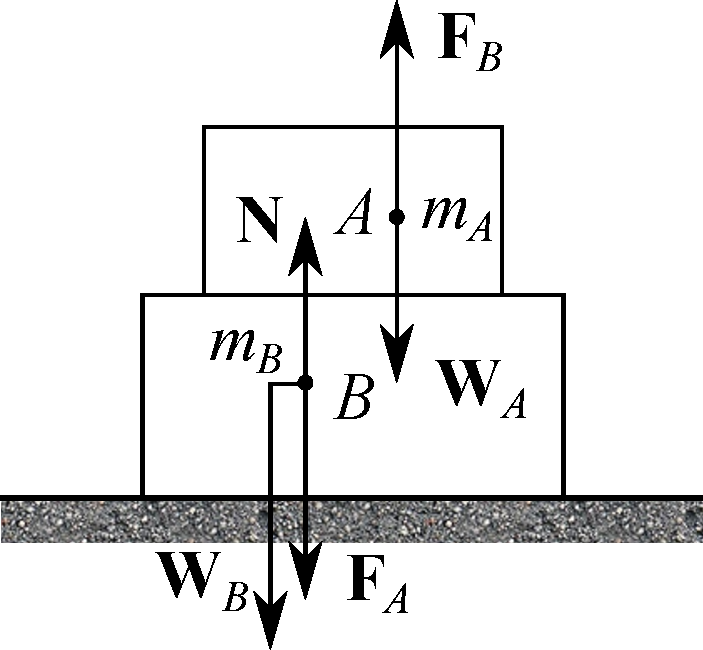
\includegraphics[scale=0.7]{blocks}
  \caption{Diagrama de fuerzas}
  \label{fig:blocks}
\end{figure}

Completando el problema de los dos bloques sobre la superficie tenemos, en la direcci\'on $\hat{\mathbf{j}}$:
\begin{align}
  \text{Ecuaciones de movimiento}&
  \begin{cases}
F_B-W_A=m_A a_A\\
N-F_A-W_B=m_B a_B\\
  \end{cases}\nonumber\\
\text{Tercera ley de Newton}\quad &F_A=F_B\nonumber\\
\text{Constraint equations}&
\begin{cases}
a_A=0\\
a_B=0\\  
\end{cases}
\end{align}
Solucionando las ecuaciones encontramos
\begin{align}
  F_B=&F_A=W_A\nonumber\\
  N=&W_A+W_B\,.
\end{align}
El objetivo principal de este ejemplo es ayudar a distinguir entre la fuerza que se aplica a un objeto 


\begin{itemize}
\item[\textbf{Ejemplo:}] Dos astronautas inicialmente en reposo en el espacio libre, tiran de ambos lados de una cuerda. La fuerza con la que el astronauta $A$ puede tirar de la cuerda, $F_A$ es mayor que la del astronauta $B$, $F_B$. Sus masas son $M_A$ y $M_B$ y la masa de la cuerda es despreciable. Encuentre el movimiento de la cuerda

Sistema: Cuerda

Entorno: Astronautas

Diagrama de cuerpo libre: (pendiente)

Ecuación de movimiento para la cuerda:
\begin{align}
  {F}_{A'}=&F_{A}\nonumber\\
  {F}_{B'}=&F_{B}
\end{align}

\begin{align}
  F_{A'}-F_{B'}=&m_{\text{cuerda}} a_{\text{cuerda}}\nonumber\\
  F_{A}-F_{B}=&m_{\text{cuerda}} a_{\text{cuerda}}\nonumber\\
\approx&0\times a_{\text{cuerda}}\nonumber\\
=&0\,,
\end{align}
de donde
\begin{align}
  F_A=F_B
\end{align}
y no hay movimiento neto de la cuerda.
\end{itemize}

\section{Ingredientes de problemas de dinámica}

\subsection{El peso}
Como hemos visto en la definción de la segundo Ley de Newton, la masa es una medidad de la resistencia que un cuerpo ofrece a los cambios en su velocidad. En la expresión para la segunda Ley de Newton con masa constante
\begin{align}
  \mathbf{F}=m_I \mathbf{a}\,,
\end{align}
$m_I$ es la masa inercial. Es el valor númerico que se obtiene al tirar un cuerpo desplazandose en una superficie sin fricción con un dinanómetro. Si simplemente se sostiene el mismo peso con un dinanómetro sobre la superficie de la tierra, obtenemos la masa gravitacional
\begin{align}
  \mathbf{F}=&m_G\mathbf{g}&\text{donde}\qquad \mathbf{g}\approx(0,-9.8,0)\ \text{m}/\text{s}^2\,,
\end{align}
Numericamente el valor de ambas masas coinciden $m=m_I=m_G$. La proporcionalidad entre masa inercial y masa gravitacional es una hipótesis en la Mecánica Newtoniana, pero es un resultado de la Teoría General de la Relatividad. Definimos entonces el peso de una partícula como el valor de la masa gravitacional por la aceleración gravitacional
\begin{align}
  |\mathbf{W}|=mg\,.
\end{align}

Hay que tener en cuenta sin embargo, que las básculas realmente miden es la fuerza normal

\subsection{Fuerza normal}
Para que un cuerpo se mantenga sobre una superficie se requiere que su peso sea compenzado por una fuerza igual y en sentido opuesto ejercida por la superficie sobre el cuerpo. Dicha fuerza se llama la fuerza normal de la superficie y se denota con la letra $\mathbf{N}$

%introducir discusion de fuerzas interatómicas

En general la fuerza normal debe incluir la presión atmosférica. Para una cuerpo con una area $A$ expuesta a la atmosféra sobre una superficie horizontal, se tendría 
\begin{align}
 N=mg+P_a A\,, 
\end{align}
donde $P_a$ es la presión atmosférica. 
\begin{itemize}
\item[\textbf{Ejemplo}] \textbf{Tortuga dentro de un ascensor}. Suponga que una tortuga, de masa $m$, está sobre una báscula dentro de un ascensor que se mueve verticalmente con una aceleración de magnitud $a_y$. Calcule la fuerza normal sobre la tortuga ejercida por la báscula. El diagrama de fuerza se muestra en la Figura (pendiente). 

La ecuación de movimiento en la dirección $y$ es (suponiendo una aceleración en la dirección $y$ positiva), con $\mathbf{N}=(0,N,0)$, $\mathbf{F}_{\text{grav}}=(0,-mg,0)$, y $\mathbf{a}=(0,a_y,0)$
\begin{align}
  N-mg=m a_y\,,
\end{align}
de modo que
\begin{align}
  N=m(g+a_y)
\end{align}
Si $a_y=0$, $N=mg$, y la báscula entrega la masa correcta para la
tortuga, sin embargo para una $a_y$ diferente de cero, la báscula
registra una ``masa'' que puede ser mayor o menor que $m$. Para
$a_y=-g$, es decir, que el ascensor se encuentra en caída libre hacia
la superficie de la tierra $N=0$, y la báscula registra un peso cero
para la tortuga. De hecho en esta situación la tortuga se encuentra en
estado de ingravidez: Un sistema cerrado (el ascensor con su contenido
interior) en caída libre en un campo gravitacional constante, es
indistinguible de un sistema con gravedad cero, es decir, el mismo
ascensor en el espacio exterior alejado de cualquier otro cuerpo.
\end{itemize}

\subsection{Cuerdas ideales}
Una cuerda ideal es inextensible y su masa es despreciable. 
\begin{itemize}
\item[\textbf{Ejemplo}] \textbf{Cuerda no ideal}
Escriba la ecuación de movimiento para una cuerda de masa $m$ sometida a tensión a ambos lados. 

La ecuación de movimiento para eje $x$ a lo largo de la cuerda es 
\begin{align*}
  \mathbf{T}_1-\mathbf{T}_2=&m\mathbf{a}\nonumber\\
  T_1-T_2=m a\,,
\end{align*}
donde $\mathbf{T}_{1,2}=(T_{1,2},0,0)$, y $\mathbf{a}=(a,0,0)$. Si la masa de la cuerda es despreciable, entonces
\begin{align*}
  T_1=T_2\,.
\end{align*}


\end{itemize}
El concepto de masa despreciable en una cuerda ideal implica que la tensión es la misma en ambos lados de la cuerda. 

\subsection{Poleas ideales}
La masa y el radio de una polea ideal son despreciables. Esto implica que las tensiones a un lado a otro de una cuerda ideal que pasa por una polea ideal son iguales en magnitud. Una polea ideal tiene entonces la propiedad de cambiar la dirección de la tensión sobre una cuerda ideal, sin alterar su magnitud.
\subsection{Aplicaciones en entornos sin fricción}







\begin{itemize}
\item[\textbf{Ejemplo:}] Tres vagones de masa $M$ están halados con una fuerza $F$ por una locomotora. Despreciando las fuerza de fricción con los rieles, encuentre las fuerzas en cada carro.
  \begin{enumerate}
  \item Sistema: Los tres vagones\\
  Entorno: los rieles y el aire\\
Diagrama: (pendiente)
  \begin{align}
    F=3M a\,,
  \end{align}
de donde
\begin{align}
  a=\frac{F}{3M}
\end{align}
\item Sistema: Primer vagón\\
Entorno: Segundo vagón, rieles, aire\\
Diagrama: (pendiente)

  \end{enumerate}
\end{itemize}
\section{Fricci\'on}

Se define como fuerza de fricción a la fuerza entre dos superficies de contacto que se opone al movimiento entre ambas superficies (\emph{fuerza de fricción dinámica}, o la fuerza que se opone al inicio del movimiento (\emph{fuerza de fricción estática}. Aunque los procesos interatómicos que dan lugar a la fuerza de fricción son muy complicados se han logrado establecer las siguientes fórmulas empíricas para la fuerza de fricción entre dos superficies

\subsection{Fricci\'on din\'amica}
\begin{align}
  \mathbf{f}=\mu_d \mathbf{N}\,,
\end{align}
donde $\mathbf{N}$, es la fuerza normal entre las superficies. El coeficiente de fricción $\mu_d$ tiene que ser menor que 1 porque de lo contrario los cuerpos se podrían subir por las paredes. 

\subsection{Fricción estática}
\begin{align}
  f>\mu_e N\,,
\end{align}
y $\mu_e$ es el coeficiete de fricción estático.




\begin{frame}
  \begin{block}%
{Ferrocarriles:} En efecto, el origen del término ferrocarril son los carriles (1) de hierro, aunque hoy en día tanto el carril como la rueda se fabrican de acero porque este material presenta unas características mecánicas más apropiadas. Además de la interesante cualidad de no tener que arreglar pinchazos (festival del humor), la principal ventaja de un transporte basado en la rodadura entre aceros es el bajo coeficiente de rozamiento que permite que un tren circulando a 100 km/h a la deriva en una vía recta y horizontal, recorra unos 10 km sin detenerse. 
  \end{block}
El coeficiente de resistencia de rodado del acero en un riel varía entre 0.0002 y 0.0010\footnote{\url{http://www.tribology-abc.com/abc/cof.htm}} 
\end{frame}

Una discusión acerca de la física de los ferrocarriles puede encontrarse en \url{http://www.jotdown.es/2012/04/el-ferrocarril-ese-gran-desconocido/}.

\begin{table}
   \centering
   \begin{tabular}{|l|c|c|}\hline
    Superficies & $\mu_e$ & $\mu_d$\\\hline
     Acero-Acero & 0.15 & 0.07\\\hline
   \end{tabular}
  \caption{Coeficientes de Fricción}
   \label{tab:coeffric}
\end{table}


\begin{itemize}
\item[Ejemplo] \textbf{Acero-Acero: Ferrocarriles} Calcule la distancia de frenado de un tren asumiendo que las ruedas dejan de rotar inmediatamente cuando se mueve a 160~Km/h.

Asumiendo que la fuerza de fricción es constante, tenemos una desaceleración constante de
\begin{align}
  a=&-\frac{f_d}{m_{\text{tren}}}=-\frac{\mu N}{m_{\text{tren}}}=-\frac{\mu m_{\text{tren}} g}{m_{\text{tren}}}=
-\mu g\,.
\end{align}
Aplicando las ecuaciones para movimiento a aceleración constante, en particular la ec.~\eqref{eq:trayectoriay}, tenemos que cuando la rapidez final es cero
\begin{align}
  v^2-v^2_0=&2 a x\nonumber\\
  -v^2_0=&2 a x\,.
\end{align}
La distancia recorrida desde el inicio del frenado es
\begin{align}
  x=&-\frac{v^2_0}{2a}\nonumber\\
 =&\frac{v_0^2}{2\mu g}\,,
\end{align}
Para $\mu_d=0.07$, tenemos $x\approx 1440\ $m.

La ley empírica de frenado de trenes es:
\begin{align}
  x=\frac{3}{2}\frac{v_0^2}{|a|}
\end{align}
donde $a$ es la desaceleración del tren, típicamente alrededor de $-2\ \text{m}/\text{s}^2$, de donde podemos obtner un estimado para el coeficiente de fricción
\begin{align*}
  \mu=\frac{|a|}{3g}=0.07\,.
\end{align*}

de donde 
\end{itemize}

\begin{itemize}
\item[\textbf{Ejemplo:}] Considere la situación ilustrada en la figura~\ref{fig:poleaideal}, donde $m_1>\mu_d m_2$. 

\begin{frame}
  \begin{figure}
    \centering
    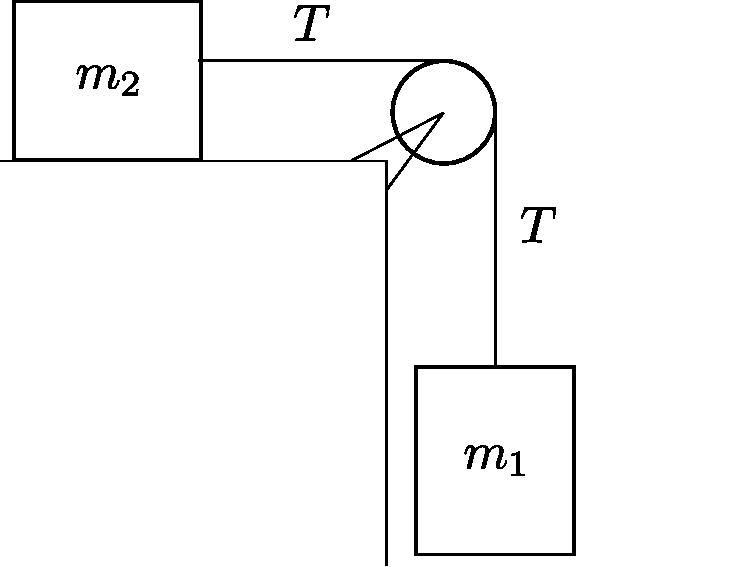
\includegraphics[scale=0.5]{poleaideal}
    \caption{Polea ideal}
    \label{fig:poleaideal}
  \end{figure}
Argumente por que la siguiente solución para la aceleración del sistema es incorrecta
\begin{align*}
      a=&\frac{g(m_1-\mu_k m_2)}{m_2-m_1}\,.
\end{align*}
\end{frame}

Con la resta en el denominador la aceleración puede ser mayor que $g$ (incluso infinita en el caso $m_1=m_2$) lo cual no tiene sentido físico.

\end{itemize}

\section{Problemas resueltos}

\ejercicio{}
\begin{frame}
  Un jugador de baloncesto lanza un balón hacia un segundo
jugador, con una rapidez $v_0$ formando un ángulo $\theta$ por
encima de la horizontal. 
En ese instante el receptor, que está a una distancia $x_0$ adelante
del lanzador, va al encuentro del balón con cierta rapidez $v_1$
constante para atraparlo a la misma altura a la cual fue lanzado.
\begin{enumerate}
\item Haga un diagrama ilustrativo de la situación planteada, donde se muestre el sistema de referencia a emplear, la trayectoria seguida por el balón y la posición inicial del receptor.
  \label{item:1jug}
\item Plantee las ecuaciones cinemáticas de posición y velocidad que rigen el movimiento del balón y del receptor.
  \label{item:2jug}
\item Encuentre el valor de la rapidez del receptor que le permite atrapar el balón. 
  \label{item:3jug}
\item Calcule la rapidez $v_1$ hallada en el literal anterior para los valores particulares de $\theta=30^\circ$ , $v_0=\SI{20}{\meter\per\second}$  y $x_0=\SI{20}{\meter}$. De acuerdo con su resultado, ¿en qué sentido se mueve el receptor?.
  \label{item:4jug}
\end{enumerate}
\end{frame}


\subsection*{Solución}
  \begin{itemize}
  \item[~\ref{item:1jug})] Escogemos el sistema de referencia en el origen del primer jugador
  \item[~\ref{item:2jug})] Para el balón
    \begin{align*}
      y=&v_{0y}t-\frac{1}{2}gt^2\nonumber\\
      x=&v_{0x}t\,.
    \end{align*}
    Para el receptor
    \begin{align*}
      x_r=&x_0+v_1 t
    \end{align*}
  \item[~\ref{item:3jug})]
    El tiempo de vuelo $t_v$ del balón se encuentra para $y=0$
    \begin{align*}
      v_{0y}t_v=&\frac{1}{2}gt_v^2\nonumber\\
      v_{0y}=&\frac{1}{2}gt_v\,,
    \end{align*}
    de modo que
    \begin{align}
      \label{eq:tv}
      t_v=&\frac{2v_{0y}}{g}\,,
    \end{align}

    Para el tiempo de vuelo $t_v$, obtenemos el alcance
    \begin{align}
      \label{eq:13}
      R=&v_{0x}t_v \nonumber\\
       =&2 v_{0x}\frac{v_{0y}}{g} \nonumber\\
       =&\frac{2 v_{0}^2\cos\theta\sin\theta}{g} \nonumber\\
       =&\frac{v_0^2}{g}\sin(2\theta)
    \end{align}
    Para que el receptor pueda atrapar el balón, su posición con respecto al sistema de referencia después de un tiempo $t_v$ debe ser justo el alcance $R$
    \begin{align*}
      x_0+v_1 t_v=&R\nonumber\\
      v_1 t_v=&\frac{v_0^2}{g}\sin(2\theta)-x_0\nonumber\\
      2 v_1 \frac{v_{0y}}{g}=&\frac{v_0^2}{g}\sin(2\theta)-x_0\nonumber\\
      v_1 =&\left( \frac{v_0^2}{g}\sin(2\theta)-x_0 \right) \frac{g}{2v_0\sin\theta}\nonumber\\
      =&\frac{v_0^2\sin(2\theta)-gx_0}{2v_0\sin\theta}\nonumber\\
    \end{align*}

    
  \item[~\ref{item:4jug})]Evaluando la ec.~(\ref{eq:v1})
    \begin{align*}
      v_1=\SI{7.52}{\meter\per\second}
    \end{align*}

además 
\begin{align*}
t_v=&\SI{2.04}{\second}\nonumber\\
 R=&\SI{35.35}{\meter}\,
\end{align*}

y el receptor se mueve en la misma dirección del balón.\finejemplo
  \end{itemize}



\ejercicio{}
\begin{frame}
 Una cuerda ideal pasa a través de una polea ideal con uno de sus
  extremos unido al bloque 1 que cuelga sobre un lado de la mesa que
  sostiene la polea. El otro extremo de la cuerda esta unido a un
  bloque 2 que se desliza a lo largo de la mesa. Ver Figura
  \ref{fig:poleaideal}. El coeficiente de fricción cinético entre la
  masa y el bloque 2 es $\mu_d$. El bloque 1 tiene una masa $m_1$ y el
  bloque 2 tiene una masa $m_2$, con $m_1>\mu_k m_2$. En el tiempo
  $t=0$, los bloques son liberados desde el reposo y la cuerda no se
  desliza alrededor de la polea, En el tiempo $t=t_1$, el bloque 1
  golpea el piso. Encuentre la magnitud de la aceleración de cada
  bloque. Exprese su respuesta en términos de $m_1$, $m_2$, $\mu_d$. 
\end{frame}

\subsubsection*{Solución}
\begin{frame}[fragile,allowframebreaks]
\begin{itemize}
\item  \textbf{Escogencia del sistema}. Para el sistema compuesto por el bloque 2, el entorno es la mesa y la cuerda, mientras que para el sistema compuesto por el bloque 1, el entorno es la cuerda y la tierra. Además escogemos un sistema de referencia $x-y$ usual. 

\item \textbf{Diagramas de fuerzas} De acuerdo a los diagramas de cuerpo libre para ambos cuerpos ilustrado en la figura~\ref{fig:poleaidealfzas}. Tenemos
  \begin{itemize}
  \item Fuerzas en $x$ bloque 2:
  \begin{align}
    \label{eq:pi1}
    (T-{\color{red}f})\hat{\mathbf{i}}=&m_2 (a\,\hat{\mathbf{i}})\nonumber\\
    T-{\color{red}f}=&m_2 a\,.
  \end{align}
  \item Fuerzas en $y$ bloque 2:
  \begin{align}
    (N-W_2)\hat{\mathbf{j}}=&0\nonumber\\
    N-W_2=&0\nonumber\\
    N=&m_2 g\,
  \end{align}
  en adelante suprimiremos los vectores unitarios en las ecuaciones
  resultantes de los diagramas de cuerpo libre.

  \item Fuerzas en $y$ bloque 1:
  \begin{align}
    \label{eq:pi2}
    T-W_1=&{\color{blue}-}m_1 a\nonumber\\
    T-m_1 g=&{\color{blue}-}m_1 a
  \end{align}
   donde el signo menos se debe a que la aceleración está en la dirección opuesta a $y$
  \end{itemize}
\item \textbf{Establezca las condiciones de ligadura:} La relación entre la fuerza normal y la fuerza de fricción es
  \begin{align}
    \label{eq:pi3}
    {\color{red}f}=&{\color{red}\mu_d} N\nonumber\\
    =&{\color{red}\mu_d} m_2 g\,.
  \end{align}
\item \textbf{Solucine las ecuaciones:} Restando las ecuaciones \eqref{eq:pi1} y \eqref{eq:pi2}, tenemos
  \begin{align*}
    -f+m_1 g=m_2 a+m_1 a=(m_2{\color{blue}+}m_1)a\,.
  \end{align*}
Despejando $a$ y usando \eqref{eq:pi3}
\begin{align}
  \label{eq:polea}
  a=&\frac{m_1g-f}{m_2{\color{blue}+}m_1}\nonumber\\
  =&\frac{m_1g-{\color{red}\mu_d} m_2 g}{m_2{\color{blue}+}m_1}\nonumber\\
  =&\frac{m_1-{\color{red}\mu_d} m_2 }{m_2{\color{blue}+}m_1}g\\
  \le&g\nonumber\,.
\end{align}
\finejemplo
\end{itemize}
%incluir aceleración


\begin{figure}
    \centering
    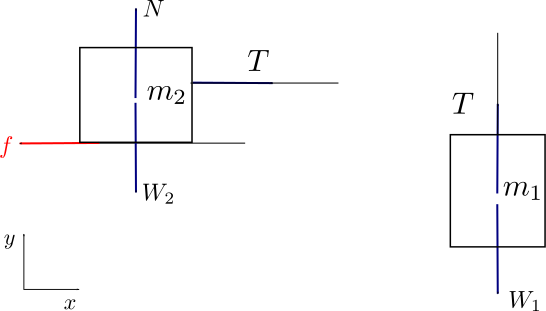
\includegraphics[scale=0.5]{poleaidealfzas}
    \caption{Diagramas de cuerpo libre ideal}
    \label{fig:poleaidealfzas}
  \end{figure}
\end{frame}
  \begin{itemize}
  \item[\textbf{Ejercicio}] Repita el problema usando un sistema de referencia rotado 90 grados en la dirección de las manecillas del reloj, para el bloque de masa $m_1$.
  \end{itemize}

\ejercicio{}

(Tomado de \cite{gabriel}) Se coloca un bloque de masa $m_1$ sobre un bloque de masa $m_2$ (como se muestra en la figura). Los coeficientes de fricción cinético y estático entre los bloques son $\mu_k$ y $\mu_e$ respectivamente. Suponer que no hay fricción entre el bloque de masa $m_2$ y la superficie sobre la cual reposa. Se aplica una fuerza $\mathbf{F}$ horizontal al bloque de masa $m_2$

  \begin{minipage}{0.4\linewidth}
    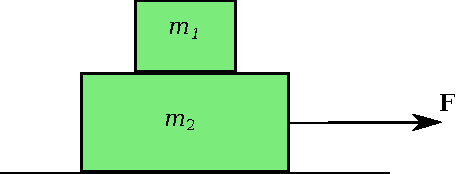
\includegraphics[scale=0.95]{bloques}
  \end{minipage}
  \begin{minipage}{0.6\linewidth}
    \begin{enumerate}
    \item Dibujar todas las fuerzas que actúan sobre cada bloque.
      \label{item:d1a}
    \item Escribir las ecuaciones de movimiento para cada bloque
      \label{item:d1b}
    \item ¿Cuál es la máxima fuerza que puede aplicarse al bloque $m_2$ de modo que los bloques se muevan juntos?
      \label{item:d1c}
    \item ¿Cual es la aceleración cuando se aplica la fuerza máxima?
      \label{item:d1d}
    \item ¿Que distancia recorren los bloques a esa aceleración durante dos segundos?
      \label{item:d1e}
    \item Evalue sus respuestas para $m_1=3\ $Kg, $m_2=5\ $Kg, $\mu_k=0.1$, $\mu_e=0.2$
      \label{item:d1f}
    \end{enumerate}
  \end{minipage}

\subsubsection*{Solución}
  \begin{itemize}
  \item[\ref{item:d1b})] Para $m_1$
    \begin{align}
      \label{eq:d11}
      m_1 a_1=&f & N_1-m_1 g=0
    \end{align}
Para $m_2$
\begin{align*}
  m_2 a_2=&F-f & N_2-N_1-m_2g=&0\,.
\end{align*}
    De modo que
    \begin{align*}
      a_1=&\frac{f}{m_1}& a_2=&\frac{F-f}{m_2}\,,
    \end{align*}
    y
    \begin{align*}
      f=\mu m_1 g\,.
    \end{align*}
  \item[\ref{item:d1c})]
    La condición de que los bloques se muevan juntos corresponde a $a_1=a_2$:
    \begin{align*}
      \frac{f}{m_1}=&\frac{F-f}{m_2}\\
      m_2 f =&m_1(F-f)\\
      m_1F =&f(m_1+m_2)\\
      m_1F =&\mu m_1 g(m_1+m_2)\\
      F =&\mu g(m_1+m_2)\,. 
    \end{align*}
    $F$ es máxima cuando $\mu=\mu_e$
    \begin{align*}
      F_{\text{max}}=\mu_e g(m_1+m_2)\,. 
    \end{align*}

    \item[\ref{item:d1d})] La aceleracíon máxima se obtiene de \eqref{eq:d11}:
      \begin{align*}
        a=\frac{f}{m_1}=\mu_e g\,.
      \end{align*}
    \item[\ref{item:d1e})] Para $t=\SI{2}{\second}$
      \begin{align*}
        x=&\frac{1}{2}a t^2
      \end{align*}
    \item[\ref{item:d1e})] $F=\SI{15.7}{\newton}$, $a=\SI{1.96}{\meter\per\second^2}$, $x=\SI{3.92}{\meter}$ \finejemplo

    \end{itemize}

\ejercicio{}
\begin{frame}[fragile,allowframebreaks]
 Dos bloques de masa $m_1$ y masa $m_2$ se mueven como lo índica la figura. Suponga que el piso es una superficie lisa (no hay fricción) y que la superficie de contacto entre los dos bloques es rugosa con coeficiente de fricción  $\mu$.

  \begin{minipage}{0.4\linewidth}
    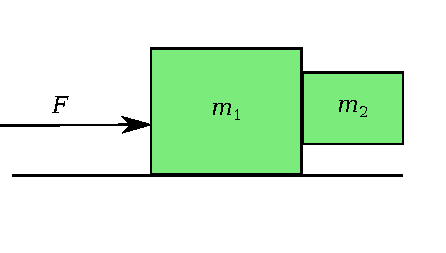
\includegraphics[scale=0.95]{bloquespegados0}
  \end{minipage}
  \begin{minipage}{0.6\linewidth}
    \begin{enumerate}
    \item Dibujar todas las fuerzas que actúan sobre cada bloque.
      \label{item:dp1a}
    \item Determine la magnitud de la fuerza mínima para que $m_2$ no se deslice. Justifique porque es mínima.
      \label{item:dp1b}
    \item Calcule dicha fuerza para $m_1=\SI{6}{\kilo\gram}$, $m_2=3\times 10^3\si{\gram}$, y $\mu=0.6$
      \label{item:dp1c}
    \end{enumerate}
  \end{minipage}
\end{frame}
\subsubsection*{Solución}
\begin{frame}[fragile,allowframebreaks]
\begin{itemize}
  \item[\ref{item:dp1a})] Recapitulemos de nuevo los pasos para solucionar los problemas de dinámica, pues en este caso son muy importantes la ecuaciones de ligadura. Primero establecemos los diagramas de cuerpo libre:
 
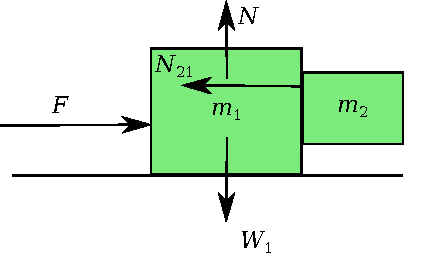
\includegraphics{bloquespegados1} 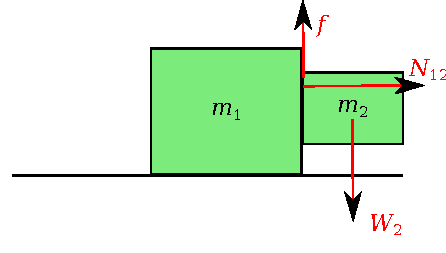
\includegraphics{bloquespegados2}

  \item[\ref{item:dp1b})] Continuamos estableciendo las ecuaciones de movimiento en forma vectorial.  


La sumatoria de fuerzas para $m_1$
    \begin{align*}
    \sum \mathbf{F}=&(F,0,0)-(N_{21},0,0)+(0,N,0)-(0,W_1,0)=(m_1 a_x,0,0)\,,  
    \end{align*}
    donde $N_{21}$ es la fuerza de reacción del bloque 2 sobre el bloque 1, de modo que la ecuación de movimiento relevante es
    \begin{align}
      \label{eq:dp1}
      F-N_{21}=&m_1 a_x\,.
    \end{align}

    Para el bloque 2 tenemos
    \begin{align*}
    \sum \mathbf{F}=&(N_{12},0,0)+(0,f,0)-(0,W_2,0)=(m_2a_x,-m_2 a_y,0)\,. 
    \end{align*}
    que da lugar a
    \begin{align}
      \label{eq:dp2}
      \sum F_x:\quad&N_{12}=m_2 a_x\nonumber\\
      \sum F_y:\quad&f-W_2=-m_2 a_y\,.
    \end{align}

    \textbf{Condiciones de ligadura}
    Para este problema podemos establecer tres condiciones de ligadura
    \begin{enumerate}
    \item $f=\mu N_{12}$, donde $N_{12}$ es la fuerza normal del bloque 1 sobre el 2.
    \item $a_y=0$, para que el bloque $m_2$ no deslice.
    \item $N_{12}=N_{21}$: los pares acción reacción son iguales en magnitud (los signos ya se tuvieron en cuenta en las respectivas ecuaciones de movimiento)
    \end{enumerate}

    Reemplazando las ecuaciones de ligadura en las ecs.~\eqref{eq:dp2}, tenemos
    \begin{align*}
      \mu N_{12}-m_2g=&0\nonumber\\
      \mu N_{21}=&m_2g\,.
    \end{align*}
    de modo que 
    \begin{align*}
    N_{21}=N_{12}=&m_2\frac{g}{\mu}\,.
    \end{align*}
    \begin{align*}
    a_x=\frac{N_{12}}{m_2}=&\frac{g}{\mu}\,.
    \end{align*}

    Reemplazando en \eqref{eq:dp1}, tenemos
    \begin{align}
      \label{eq:dp4}
      F_{\text{min}}=&N_{21}+m_1 a_x\nonumber\\
      =&m_2\frac{g}{\mu}+m_1 \frac{g}{\mu}\nonumber\\
      =&(m_1+m_2)\frac{g}{\mu}\,.
    \end{align}

    \item[\ref{item:d1b})] Evaluando numéricamente tenemos que
      \begin{align*}
        F_{\text{min}}=\SI{147}{\newton}\,.
      \end{align*}

      Como un chequeo de consistencia, podemos ver de \eqref{eq:dp4}
      \begin{align*}
        F_{\text{min}}=&(m_1+m_2)\frac{g}{\mu}\nonumber\\
        =&(m_1+m_2)a_x\,.
      \end{align*}
      de modo que el sistema completo de los dos bloques, dentro del
      cual se cancelan todas las fuerzas internas, se mueve como un
      sistema de masa $m_1+m_2$ bajo el efecto de la fuerza externa
      $F_{\text{min}}$.\finejemplo

\end{itemize}
\end{frame}

\ejemplo{}
Considere dos bloques de masas $m_1$ y $m_2$ unidos por 
una cuerda inextensible de longitud $d$. El primer bloque está en un 
superficie horizontal sin fricción y el segundo desciende desde el reposo
por un plano inclinado también sin fricción que forma un ángulo $\theta$ 
con la horizontal. Cuando el bloque 2 llega al piso, después de deslizar
una distancia $d$, este para súbitamente debido a una cuña, y el bloque 1 
queda con una velocidad horizontal y cae en un movimiento parabólico 
(la cuerda no ejerce ningún efecto en la caída parabólica).

  \begin{minipage}{0.4\linewidth}
    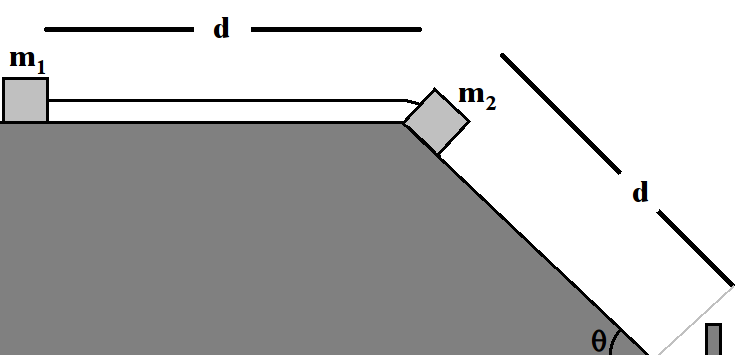
\includegraphics[scale=0.4]{Punto2.png}
  \end{minipage}
  \begin{minipage}{0.6\linewidth}
    \begin{enumerate}
    \item Realice un diagrama de cuerpo libre de cada bloque en 
la situación inicial.
\item Demuestre que la rapidez final del bloque 2 cuando llega 
al piso es

\[ v_f = \sqrt{ \frac{2dm_2g\sin \theta}{m_1+m_2} } \]

\label{item:bbc1}
\item Calcule el alcance horizontal del bloque 1 cuando cae
al piso.
\label{item:bbc2}
\item Determine la razón de masas $m_1/m_2$ en términos de 
$\theta$ y $d$, necesaria para que el bloque 1 caiga justo sobre el bloque 2.
\label{item:bbc3}
\end{enumerate}
\end{minipage}

\textbf{Solución}
  \begin{itemize}
  \item[\ref{item:bbc1})] La aceleración del bloque $m_2$ se obtiene de
    \begin{align}
      T=&m_1 a \nonumber\\
      -T+m_2g\sin\theta=&m_2 a
    \end{align}
de modo que
\begin{align}
  a=&g\frac{m_2\sin\theta}{m_1+m_2}\,,
\end{align}
La rapidez final después de recorrer una distancia $d$ es
\begin{align}
  v_f=&\sqrt{2da}\nonumber\\
   =&\sqrt{\frac{2dm_2g\sin\theta}{m_1+m_2}}\,.
\end{align}
\item[\ref{item:bbc2})] Esta es la rapidez inicial del bloque en la
  dirección horizontal (ángulo de lanzamiento $\alpha=0$) de $m_1$ al
  salir de la superficie horizontal.
  Por lo tanto, el alcance horizontal es la distancia recorrida en el
  tiempo de vuelo, que tomando como origen de coordenadas la base del
  plano inclinado y teniendo en cuenta la rapidez inicial en $y=0$, es
\begin{align}
 y_{f}=0=&d\sin\theta-\frac{1}{2}g t_{\text{vuelo}}^2
\end{align}
\begin{align}
  t_{\text{vuelo}}=\sqrt{\frac{2d\sin\theta}{g}}
\end{align}
y por consiguiente, el alcance en $x$ es
\begin{align}
  x=&v_{0x}t_{\text{vuelo}}\nonumber\\
   =&v_f t_{\text{vuelo}}\nonumber\\
   =&\sqrt{\left(\frac{2dm_2g\sin\theta}{m_1+m_2}\right)\left(\frac{2d\sin\theta}{g}\right)}\nonumber\\
   =&2d\sin\theta\sqrt{\frac{m_2}{m_1+m_2}}\,,
\end{align}
\item[\ref{item:bbc3})] La condición implica que
  \begin{align}
    d\cos\theta=&x \nonumber\\
               =&2d\sin\theta\sqrt{\frac{m_2}{m_1+m_2}}\,,
  \end{align}
de modo que
\begin{align}
\sqrt{\frac{m_1+m_2}{m_2}}=&2\tan\theta \nonumber\\
\frac{m_1+m_2}{m_2}=&4\tan^2\theta \nonumber\\
\frac{m_1}{m_2}=&4\tan^2\theta-1\,.
\end{align}


  \end{itemize}
    




\subsubsection*{Ejercicio}
Calcule la aceleración con la que cae el bloque 2 para un determinado valor de la fuerza aplicada $F$.

\ejercicio{}
Un bloque de masa $m_{1}$ está unido a una masa $m_{2}$ por medio de una cuerda inextensible, como lo indica la figura. Desprecie la fricción entre el bloque y el plano inclinado. El ángulo de inclinación del plano es $\theta$ con respecto a la horizontal. Suponga que la polea es ideal.

\begin{minipage}{12 cm}{
\begin{enumerate}
\item Dibujar todas las fuerzas que actúan sobre $m_{1}$ y $m_{2}$.
\item Escoja el sistema de referencia que considere adecuado para cada una de las masas y 
escriba  las   ecuaciones   de movimiento, tanto para $m_{1}$, como  para $m_{2}$.
\item Calcular la aceleración de las masas y la tensión en la cuerda en términos de $m_{1}$, $m_{2}$, $g$ y $\theta$.

\item Finalmente use la calculadora y calcule los valores numéricos si $m_{2}=\SI{5}{\kilo\gram}$, $m_{1}=\SI{2}{\kilo\gram}$, y $\theta=30^\circ$. 
\end{enumerate}
}\end{minipage}
\begin{minipage}{6 cm}{
\begin{center}
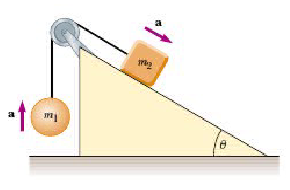
\includegraphics[scale=0.6]{planoinclinado}
\end{center}
}\end{minipage}


  Respuestas:
  \begin{align*}
    a=\dfrac{g}{(m_{1}+m_{2})}[m_{2}(-\mu \cos\theta +\sin\theta) - m_{1}]
  \end{align*}   
 \begin{align*}
   T=g\dfrac{m_{1}m_{2}}{(m_{1}+m_{2})}[1-\mu\cos\theta + \sin\theta]
\end{align*}




% \begin{extrapage}
%   \newpage
%   \qquad
%   \newpage
% \end{extrapage}

%%% Local Variables: 
%%% mode: latex
%%% TeX-master: "mecanica"
%%% End: